%2multibyte Version: 5.50.0.2960 CodePage: 65001
% !TeX root = ./Slides_Lez_02_Variabili_Casuali.tex
% **********************
% Macro matematiche ufficiali del progetto MQF
% Coerenti con MQF_Notazione.tex
% **********************
% Fallback utile per compilazione esterna se qualche titolo resta scritto come \QTR.
% Scientific WorkPlace usa \QTR internamente; in Beamer \QTR{frametitle}{Titolo}
% deve espandersi in \frametitle{Titolo}.
%\usepackage{hyperref}

\documentclass[handout]{beamer}%
\usepackage{mathpazo}
\usepackage{multimedia}
\usepackage{amsmath}
\usepackage{amsfonts}
\usepackage{amssymb}
\usepackage{graphicx}%
\setcounter{MaxMatrixCols}{30}
%TCIDATA{OutputFilter=latex2.dll}
%TCIDATA{Version=5.50.0.2960}
%TCIDATA{Codepage=65001}
%TCIDATA{CSTFile=beamer.cst}
%TCIDATA{Created=Saturday, May 16, 2026 09:09:59}
%TCIDATA{LastRevised=Monday, November 02, 2026 19:40:13}
%TCIDATA{<META NAME="GraphicsSave" CONTENT="32">}
%TCIDATA{<META NAME="SaveForMode" CONTENT="2">}
%TCIDATA{BibliographyScheme=Manual}
%TCIDATA{<META NAME="DocumentShell" CONTENT="Other Documents\SW\Slides - Beamer">}
%BeginMSIPreambleData
\providecommand{\U}[1]{\protect\rule{.1in}{.1in}}
%EndMSIPreambleData
\newenvironment{stepenumerate}{\begin{enumerate}[<+->]}{\end{enumerate}}
\newenvironment{stepitemize}{\begin{itemize}[<+->]}{\end{itemize} }
\newenvironment{stepenumeratewithalert}{\begin{enumerate}[<+-| alert@+>]}{\end{enumerate}}
\newenvironment{stepitemizewithalert}{\begin{itemize}[<+-| alert@+>]}{\end{itemize} }
\usetheme{Madrid}
\setbeamersize{, text margin right=5mm}
\providecommand{\R}{\mathbb{R}}
\providecommand{\N}{\mathbb{N}}
\providecommand{\E}{\mathbb{E}}
\providecommand{\Prob}{\mathbb{P}}
\providecommand{\Q}{\mathbb{Q}}
\providecommand{\F}{\mathcal{F}}
\providecommand{\B}{\mathcal{B}}
\providecommand{\G}{\mathcal{G}}
\providecommand{\1}{\mathbf{1}}
\providecommand{\Var}{\operatorname{Var}}
\providecommand{\Cov}{\operatorname{Cov}}
\providecommand{\VaR}{\operatorname{VaR}}
\providecommand{\CVaR}{\operatorname{CVaR}}
\providecommand{\argmin}{\operatorname*{arg\,min}}
\providecommand{\argmax}{\operatorname*{arg\,max}}
\providecommand{\EVPI}{\operatorname{EVPI}}
\providecommand{\VSS}{\operatorname{VSS}}
\providecommand{\QTR}[2]{\csname #1\endcsname{#2}}
%**** Cartella delle figure: percorso relativo (Overleaf) e assoluto (SWP 5.5)
\graphicspath{{../graphics/}{E:/Didattica/MQF/Github/CORSO-MQF/graphics/}}
%**** Titolo, autori e barra inferiore: campo TeX "Frontespizio" dopo \begin{document}
%BeginMSIPreambleData
\ifx\pdfoutput\relax\let\pdfoutput=\undefined\fi
\newcount\msipdfoutput
\ifx\pdfoutput\undefined\else
\ifcase\pdfoutput\else
\msipdfoutput=1
\ifx\paperwidth\undefined\else
\ifdim\paperheight=0pt\relax\else\pdfpageheight\paperheight\fi
\ifdim\paperwidth=0pt\relax\else\pdfpagewidth\paperwidth\fi
\fi\fi\fi
%EndMSIPreambleData
\begin{document}

%****************************************************************
%**** PAGINA DI TITOLO E BARRA INFERIORE (campo TeX "Frontespizio")
%**** Contiene: footline, title, subtitle, author, institute, date,
%**** titlegraphic, maketitle. Resta qui, nel corpo del documento:
%**** nel preambolo SWP 5.5 altera argomenti opzionali e fine riga.
%**** Vedi MQF_Project_Guidelines.md, sezione 10.2.
%****************************************************************
%TCIMACRO{\TeXButton{Frontespizio}{\setbeamertemplate{footline}{\leavevmode
%\hbox{\begin{beamercolorbox}[wd=.20\paperwidth
%,ht=2.25ex,dp=1ex,center]{author in head/foot}\usebeamerfont
%{author in head/foot}\insertshortauthor\end{beamercolorbox}%
%\begin{beamercolorbox}[wd=.69\paperwidth
%,ht=2.25ex,dp=1ex,center]{title in head/foot}\usebeamerfont
%{title in head/foot}\insertshorttitle\end{beamercolorbox}%
%\begin{beamercolorbox}[wd=.11\paperwidth
%,ht=2.25ex,dp=1ex,right]{date in head/foot}\usebeamerfont{date in head/foot}%
%\insertshortdate{}\hspace*{2em}\insertframenumber{} / \inserttotalframenumber
%\hspace*{2ex}\end{beamercolorbox}}\vskip0pt}\title
%[Lez. 2 - Variabili casuali e distribuzioni]{Lezione 2 - Variabili casuali e distribuzioni}%
%\subtitle{Metodi Quantitativi per la Finanza}\author
%[P. Falbo, C. Pelizzari]{{\LARGE Paolo Falbo, Cristian Pelizzari}}%
%\institute[]{{\large Dipartimento di Economia e Management}}\date
%[]{}\titlegraphic{
\includegraphics[height=1.25cm]{MQF_logo.png}\hspace
%{0.8cm}
\includegraphics[height=1.25cm]{logo-Unibs-esteso.png}}\maketitle}}%
%BeginExpansion
\setbeamertemplate{footline}{\leavevmode\hbox{\begin{beamercolorbox}%
[wd=.20\paperwidth,ht=2.25ex,dp=1ex,center]{author in head/foot}%
\usebeamerfont{author in head/foot}\insertshortauthor\end{beamercolorbox}%
\begin{beamercolorbox}[wd=.69\paperwidth
,ht=2.25ex,dp=1ex,center]{title in head/foot}\usebeamerfont
{title in head/foot}\insertshorttitle\end{beamercolorbox}%
\begin{beamercolorbox}[wd=.11\paperwidth
,ht=2.25ex,dp=1ex,right]{date in head/foot}\usebeamerfont{date in head/foot}%
\insertshortdate{}\hspace*{2em}\insertframenumber{} / \inserttotalframenumber
\hspace*{2ex}\end{beamercolorbox}}\vskip0pt}\title
[Lez. 2 - Variabili casuali e distribuzioni]{Lezione 2 - Variabili casuali e distribuzioni}%
\subtitle{Metodi Quantitativi per la Finanza}\author
[P. Falbo, C. Pelizzari]{{\LARGE Paolo Falbo, Cristian Pelizzari}}%
\institute[]{{\large Dipartimento di Economia e Management}}\date
[]{}\titlegraphic{
\includegraphics[height=1.25cm]{MQF_logo.png}\hspace
{0.8cm}
\includegraphics[height=1.25cm]{logo-Unibs-esteso.png}}\maketitle
%EndExpansion
%****************************************************************
%**** FINE PAGINA DI TITOLO
%****************************************************************


\section{Apertura}

%***********************************


\subsection{Apertura: perch\'{e} servono le variabili casuali}%

%TCIMACRO{\TeXButton{BeginFrame}{\begin{frame}}}%
%BeginExpansion
\begin{frame}%
%EndExpansion
%

%TCIMACRO{\QTR{frametitle}{Variabili casuali: dagli scenari ai valori}}%
%BeginExpansion
\frametitle{Variabili casuali: dagli scenari ai valori}%
%EndExpansion


\textbf{Idea centrale.}

\medskip

L'incertezza finanziaria diventa operativa quando agli scenari associamo
grandezze numeriche.%

\[
\omega\in\Omega\quad\longmapsto\quad X(\omega)\in\mathbb{R}
\]


\medskip

\textbf{Esempi finanziari.}%

\[%
\begin{array}
[c]{rcl}%
R(\omega) & = & \mbox{rendimento aleatorio},\\[4pt]%
L(\omega) & = & \mbox{perdita aleatoria},\\[4pt]%
S_{T}(\omega) & = & \mbox{prezzo futuro aleatorio},\\[4pt]%
H(\omega) & = & \mbox{payoff aleatorio}.
\end{array}
\]


\medskip

Gli eventi restano il fondamento probabilistico; la finanza quantitativa
lavora sui valori numerici generati dagli scenari.%

%TCIMACRO{\TeXButton{Transition: Box Out}{\transboxout}}%
%BeginExpansion
\transboxout
%EndExpansion%
%TCIMACRO{\TeXButton{EndFrame}{\end{frame}}}%
%BeginExpansion
\end{frame}%
%EndExpansion


%***********************************


\subsection{La domanda della lezione}%

%TCIMACRO{\TeXButton{BeginFrame}{\begin{frame}}}%
%BeginExpansion
\begin{frame}%
%EndExpansion
%

%TCIMACRO{\QTR{frametitle}{La domanda della lezione}}%
%BeginExpansion
\frametitle{La domanda della lezione}%
%EndExpansion


Non basta chiedere se un evento si verifica: occorre descrivere la
distribuzione dei valori assunti da una grandezza finanziaria aleatoria.%

\[
\Prob(R<0), \qquad\Prob(L>\ell), \qquad\Prob(S_{T}>K)
\]


\medskip

\textbf{Domanda guida.}

\medskip

Come si descrive probabilisticamente un rendimento, una perdita o un payoff aleatorio?%

%TCIMACRO{\TeXButton{Transition: Box Out}{\transboxout}}%
%BeginExpansion
\transboxout
%EndExpansion%
%TCIMACRO{\TeXButton{EndFrame}{\end{frame}}}%
%BeginExpansion
\end{frame}%
%EndExpansion


%***********************************


\subsection{Mappa della lezione}%

%TCIMACRO{\TeXButton{BeginFrame}{\begin{frame}}}%
%BeginExpansion
\begin{frame}%
%EndExpansion
%

%TCIMACRO{\QTR{frametitle}{Mappa della lezione}}%
%BeginExpansion
\frametitle{Mappa della lezione}%
%EndExpansion


La lezione costruisce il ponte tra probabilit\`{a} astratta e misurazione
quantitativa del rischio.%

\[
\begin{aligned}
&(\Omega,\F,\Prob)
\quad\longrightarrow\quad X
\quad\longrightarrow\quad \Prob_X,\ F_X,\ p_X,\ f_X\\[4pt]
&\quad\longrightarrow\quad \E[X],\ \Var(X),\ q_\alpha(X)
\end{aligned}
\]


\medskip%

\[%
\begin{array}
[c]{rcl}%
\Prob_{X} & : & \mbox{distribuzione indotta su $\mathbb{R}$ da } X,\\[4pt]%
F_{X} & : & \mbox{funzione di distribuzione},\\[4pt]%
p_{X} & : & \mbox{funzione di probabilit\`{a}},\\[4pt]%
f_{X} & : & \mbox{densit\`{a} di probabilit\`{a}},\\[4pt]%
\E[X],\ \Var(X),\ q_{\alpha}(X) & : &
\mbox{sintesi di posizione, dispersione e coda}.
\end{array}
\]


\medskip

Obiettivo: tradurre l'incertezza sugli scenari in strumenti operativi per
rendimenti, perdite, payoff e rischio di coda.%

%TCIMACRO{\TeXButton{Transition: Box Out}{\transboxout}}%
%BeginExpansion
\transboxout
%EndExpansion%
%TCIMACRO{\TeXButton{EndFrame}{\end{frame}}}%
%BeginExpansion
\end{frame}%
%EndExpansion


%***********************************


\subsection{Definizione di variabile casuale}%

%TCIMACRO{\TeXButton{BeginFrame}{\begin{frame}}}%
%BeginExpansion
\begin{frame}%
%EndExpansion
%

%TCIMACRO{\QTR{frametitle}{Variabile casuale: dagli scenari ai valori}}%
%BeginExpansion
\frametitle{Variabile casuale: dagli scenari ai valori}%
%EndExpansion


Una variabile casuale reale \textbf{\`{e}, in primo luogo, una funzione} che
associa un numero reale a ciascun esito dello spazio campionario:%

\[
X:\Omega\longrightarrow\mathbb{R}.
\]


\medskip

Se $\omega\in\Omega$ \`{e} uno scenario, allora $X(\omega)$ \`{e} il valore
numerico generato da quello scenario.

\medskip%

\[%
\begin{array}
[c]{rcl}%
\omega & : & \mbox{scenario possibile},\\[4pt]%
X(\omega) & : & \mbox{valore della grandezza aleatoria nello scenario }
\omega.
\end{array}
\]


\medskip

Esempi: rendimento futuro, perdita di portafoglio, prezzo futuro, payoff.%

%TCIMACRO{\TeXButton{Transition: Box Out}{\transboxout}}%
%BeginExpansion
\transboxout
%EndExpansion%
%TCIMACRO{\TeXButton{EndFrame}{\end{frame}}}%
%BeginExpansion
\end{frame}%
%EndExpansion


%***********************************


\subsection{Eventi generati da una variabile casuale}%

%TCIMACRO{\TeXButton{BeginFrame}{\begin{frame}}}%
%BeginExpansion
\begin{frame}%
%EndExpansion
%

%TCIMACRO{\QTR{frametitle}{Eventi generati da una variabile casuale}}%
%BeginExpansion
\frametitle{Eventi generati da una variabile casuale}%
%EndExpansion


\textbf{Una condizione sui valori di $X$ individua un insieme di scenari}.%

\[
\{X\leq x\} = \{\omega\in\Omega:X(\omega)\leq x\}
\]


\medskip

Analogamente,%

\[
\{X=x_{i}\} = \{\omega\in\Omega:X(\omega)=x_{i}\},
\]
%

\[
\{a<X\leq b\} = \{\omega\in\Omega:a<X(\omega)\leq b\}.
\]


\medskip

La probabilit\`{a} resta assegnata a eventi dello spazio originario:%

\[
\Prob(X\leq x) = \Prob(\{\omega\in\Omega:X(\omega)\leq x\}).
\]
%

%TCIMACRO{\TeXButton{Transition: Box Out}{\transboxout}}%
%BeginExpansion
\transboxout
%EndExpansion%
%TCIMACRO{\TeXButton{EndFrame}{\end{frame}}}%
%BeginExpansion
\end{frame}%
%EndExpansion


%***********************************


\subsection{Misurabilit\`{a}}%

%TCIMACRO{\TeXButton{BeginFrame}{\begin{frame}}}%
%BeginExpansion
\begin{frame}%
%EndExpansion
%

%TCIMACRO{\QTR{frametitle}{La condizione di misurabilit\`{a}}}%
%BeginExpansion
\frametitle{La condizione di misurabilit\`{a}}%
%EndExpansion


Una funzione $X:\Omega\to\mathbb{R}$ \`{e} una variabile casuale
\textbf{misurabile} se, per ogni $x\in\mathbb{R}$, l'evento
\[
\{X\leq x\} = \{\omega\in\Omega:X(\omega)\leq x\}
\]
appartiene alla $\sigma$-algebra $\F$ (famiglia degli eventi rilevanti).

%Una funzione $X:\Omega\to\mathbb{R}$ \`{e} una variabile casuale \textbf{misurabile} se gli eventi del tipo $\{X\leq x\}$, o, pi\`{u} precisamente, $ \{\omega \in \Omega:X(\omega)\leq x \}$,  sono inclusi nella $\sigma$-algebra $\F$, (famiglia degli eventi rilevanti):
%\[
%\{X\leq x\}\in\F
%\qquad
%\mbox{per ogni } %x\in\mathbb{R}.
%\]


\medskip

Questa condizione garantisce che la quantit\`{a}%

\[
\Prob(X\leq x)
\]


sia ben definita.

\medskip%

\[%
\begin{array}
[c]{rcl}%
X & : & \mbox{assegna valori numerici agli esiti},\\[4pt]%
\F & : & \mbox{contiene gli eventi rilevanti / osservabili},\\[4pt]%
\Prob & : & \mbox{assegna probabilit\`{a} agli eventi di } \F.
\end{array}
\]
%

%TCIMACRO{\TeXButton{Transition: Box Out}{\transboxout}}%
%BeginExpansion
\transboxout
%EndExpansion%
%TCIMACRO{\TeXButton{EndFrame}{\end{frame}}}%
%BeginExpansion
\end{frame}%
%EndExpansion


%***********************************


\subsection{Esempio guida: scenari, regimi e rendimento}%

%TCIMACRO{\TeXButton{BeginFrame}{\begin{frame}}}%
%BeginExpansion
\begin{frame}%
%EndExpansion
%

%TCIMACRO{\QTR{frametitle}{Sei scenari, tre regimi di mercato}}%
%BeginExpansion
\frametitle{Sei scenari, tre regimi di mercato}%
%EndExpansion


Consideriamo sei esiti elementari:%

\[
\Omega=\{\omega_{1},\omega_{2},\omega_{3},\omega_{4},\omega_{5},\omega_{6}\}.
\]


\medskip

Gli scenari sono raggruppati in tre regimi di mercato:%

\[
A_{1}=\{\omega_{1},\omega_{2}\}, \qquad A_{2}=\{\omega_{3},\omega_{4}\},
\qquad A_{3}=\{\omega_{5},\omega_{6}\}.
\]


\medskip%

\[%
\begin{array}
[c]{rcl}%
A_{1} & : & \mbox{regime sfavorevole},\\[4pt]%
A_{2} & : & \mbox{regime intermedio},\\[4pt]%
A_{3} & : & \mbox{regime favorevole}.
\end{array}
\]


\medskip

Idea: il modello distingue i regimi, non necessariamente ogni singolo esito elementare.%

%TCIMACRO{\TeXButton{Transition: Box Out}{\transboxout}}%
%BeginExpansion
\transboxout
%EndExpansion%
%TCIMACRO{\TeXButton{EndFrame}{\end{frame}}}%
%BeginExpansion
\end{frame}%
%EndExpansion


%***********************************


\subsection{Sigma-algebra generata dalla partizione}%

%TCIMACRO{\TeXButton{BeginFrame}{\begin{frame}}}%
%BeginExpansion
\begin{frame}%
%EndExpansion
%

%TCIMACRO{\QTR{frametitle}{Eventi osservabili nel modello}}%
%BeginExpansion
\frametitle{Eventi osservabili nel modello}%
%EndExpansion


La partizione genera la sigma-algebra degli eventi osservabili:%

\[
\F=\sigma(A_{1},A_{2},A_{3}).
\]


\medskip

Esplicitamente,%

\[
\F= \{\varnothing, A_{1},A_{2},A_{3}, A_{1}\cup A_{2},A_{1}\cup A_{3}%
,A_{2}\cup A_{3}, \Omega\}.
\]


\medskip

La sigma-algebra specifica eventi rilevanti e osservabili nel modello, ad esempio:

\medskip%

\[%
\begin{array}
[c]{rcl}%
A_{1}\cup A_{2} & : & \mbox{regime non favorevole},\\[4pt]%
A_{2}\cup A_{3} & : & \mbox{regime non sfavorevole},\\[4pt]%
... &  &
\end{array}
\]
%

%TCIMACRO{\TeXButton{Transition: Box Out}{\transboxout}}%
%BeginExpansion
\transboxout
%EndExpansion%
%TCIMACRO{\TeXButton{EndFrame}{\end{frame}}}%
%BeginExpansion
\end{frame}%
%EndExpansion


%***********************************


\subsection{Rendimento come variabile casuale}%

%TCIMACRO{\TeXButton{BeginFrame}{\begin{frame}}}%
%BeginExpansion
\begin{frame}%
%EndExpansion
%

%TCIMACRO{\QTR{frametitle}{Il rendimento come funzione degli scenari}}%
%BeginExpansion
\frametitle{Il rendimento come funzione degli scenari}%
%EndExpansion


Definiamo una variabile casuale $X$ che rappresenta il rendimento del portafoglio:%

\[
X(\omega)=
\begin{cases}
-0.04, & \mbox{se } \omega\in A_{1},\\
0.01, & \mbox{se } \omega\in A_{2},\\
0.06, & \mbox{se } \omega\in A_{3}.
\end{cases}
\]


\medskip

La variabile casuale aggrega scenari diversi nello stesso valore numerico:%

\[%
\begin{array}
[c]{rcl}%
\{X=-0.04\} = A_{1}, \qquad\{X=0.01\} = A_{2},\qquad\{X=0.06\} = A_{3}. &  &
\end{array}
\]


\medskip

Esempi di eventi generati da $X$:%

\[
\{X<0\}=A_{1}, \qquad\{X\geq0.01\}=A_{2}\cup A_{3}.
\]


\medskip

La condizione numerica su $X$ individua un evento appartenente a $\F$.%

%TCIMACRO{\TeXButton{Transition: Box Out}{\transboxout}}%
%BeginExpansion
\transboxout
%EndExpansion%
%TCIMACRO{\TeXButton{EndFrame}{\end{frame}}}%
%BeginExpansion
\end{frame}%
%EndExpansion


%***********************************


\subsection{Controimmagini, Borel e distribuzione indotta}%

%TCIMACRO{\TeXButton{BeginFrame}{\begin{frame}}}%
%BeginExpansion
\begin{frame}%
%EndExpansion
%

%TCIMACRO{\QTR{frametitle}{Controimmagini: dai valori agli eventi}}%
%BeginExpansion
\frametitle{Controimmagini: dai valori agli eventi}%
%EndExpansion


Sia $X:\Omega\to\mathbb{R}$ una funzione e sia $B\subseteq\mathbb{R}$.

\medskip

La controimmagine di $B$ mediante $X$ \`{e}%

\[
X^{-1}(B)=\{\omega\in\Omega:X(\omega)\in B\}.
\]


\medskip

Essa \`{e} un sottoinsieme di $\Omega$, quindi un candidato evento.

\medskip

Esempi:%

\[
X^{-1}((-\infty,x]) = \{\omega\in\Omega:X(\omega)\leq x\} = \{X\leq x\},
\]
%

\[
X^{-1}((a,b]) = \{\omega\in\Omega:a<X(\omega)\leq b\} = \{a<X\leq b\}.
\]


\medskip

%(la notazione $X^{-1}(B)$ non \`{e} da intendersi nel senso abituale, ma come mappa che lavora in direzione inversa alla v.c. $X$).


(la notazione $X^{-1}(B)$ indica la controimmagine di $B$ tramite $X$ e non
richiede che la funzione $X$ sia invertibile).%

%TCIMACRO{\TeXButton{Transition: Box Out}{\transboxout}}%
%BeginExpansion
\transboxout
%EndExpansion%
%TCIMACRO{\TeXButton{EndFrame}{\end{frame}}}%
%BeginExpansion
\end{frame}%
%EndExpansion


%***********************************


\subsection{Il ruolo della sigma-algebra boreliana}%

%TCIMACRO{\TeXButton{BeginFrame}{\begin{frame}}}%
%BeginExpansion
\begin{frame}%
%EndExpansion
%

%TCIMACRO{\QTR{frametitle}{Il ruolo di $\QTR{cal}{B}(\QTR{Bbb}{R})$}}%
%BeginExpansion
\frametitle{Il ruolo di $\mathcal{B}(\mathbb{R})$}%
%EndExpansion


Per variabili casuali reali, gli eventi sui valori di $X$ sono sottoinsiemi
della retta reale.

\medskip

La classe naturale di tali insiemi \`{e} la sigma-algebra boreliana:%

\[
\mathcal{B}(\mathbb{R}).
\]


\medskip

Essa contiene gli insiemi normalmente usati per descrivere eventi sui valori reali:%

\[
(-\infty,x], \qquad(a,b], \qquad[a,b], \qquad(x,+\infty).
\]


\medskip

La misurabilit\`{a} richiede:%

\[
B\in\mathcal{B}(\mathbb{R}) \quad\Longrightarrow\quad X^{-1}(B)\in\F.
\]


\medskip

Quindi ogni condizione boreliana sui valori di $X$ genera un evento
osservabile nello spazio originario.%

%TCIMACRO{\TeXButton{Transition: Box Out}{\transboxout}}%
%BeginExpansion
\transboxout
%EndExpansion%
%TCIMACRO{\TeXButton{EndFrame}{\end{frame}}}%
%BeginExpansion
\end{frame}%
%EndExpansion


%***********************************


\subsection{Distribuzione indotta}%

%TCIMACRO{\TeXButton{BeginFrame}{\begin{frame}}}%
%BeginExpansion
\begin{frame}%
%EndExpansion
%

%TCIMACRO{\QTR{frametitle}{Distribuzione indotta da una variabile casuale}}%
%BeginExpansion
\frametitle{Distribuzione indotta da una variabile casuale}%
%EndExpansion


La variabile casuale $X$ \textbf{trasferisce} o \textbf{induce} la
probabilit\`{a} da $\Omega$ alla retta reale. Ci\`{o} \`{e} possibile grazie
alla \textbf{misura di probabilit\`{a} indotta} $\Prob_{X}$:
\[
\Prob_{X}:=\Prob\circ X^{-1}
\]
ossia, per ogni $B \in\mathcal{B}(\mathbb{R})$,
\[
\Prob_{X}(B) = \Prob\left( X^{-1}(B)\right) .
\]
Con la differenza che
\[%
\begin{array}
[c]{ccc}%
B\subseteq\mathbb{R} & \longmapsto & X^{-1}(B)\subseteq\Omega\\[5pt]%
\mbox{insieme di valori} &  & \mbox{evento nello spazio campionario}
\end{array}
\]
%

\[%
\begin{array}
[c]{rcl}%
\Prob & : & \mbox{probabilit\`{a} sugli eventi di } \Omega,\\[4pt]%
\Prob_{X} & : & \mbox{probabilit\`{a} indotta sui valori reali di } X.
\end{array}
\]


\medskip

Messaggio: la misura $\Prob_{X}$ \`{e} importante perch\'{e} costituisce la
\textbf{distribuzione} di $X$, cio\`{e} la collezione delle probabilit\`{a} di
tutti i possibili eventi $\{X\in B\}$.%

%TCIMACRO{\TeXButton{Transition: Box Out}{\transboxout}}%
%BeginExpansion
\transboxout
%EndExpansion%
%TCIMACRO{\TeXButton{EndFrame}{\end{frame}}}%
%BeginExpansion
\end{frame}%
%EndExpansion


%***********************************


\subsection{Funzione di distribuzione}%

%TCIMACRO{\TeXButton{BeginFrame}{\begin{frame}}}%
%BeginExpansion
\begin{frame}%
%EndExpansion
%

%TCIMACRO{\QTR{frametitle}{Funzione di distribuzione}}%
%BeginExpansion
\frametitle{Funzione di distribuzione}%
%EndExpansion


La distribuzione di una variabile casuale reale pu\`{o} essere rappresentata
mediante la funzione di distribuzione.%

\[
F_{X}(x) = \Prob_{X}((-\infty,x]) = \Prob(X\leq x), \qquad x\in\mathbb{R}.
\]


\medskip

$F_{X}(x)$ misura la probabilit\`{a} cumulata fino alla soglia $x$.

\medskip%

\[%
\begin{array}
[c]{rcl}%
x & : & \mbox{soglia reale},\\[4pt]%
\{X\leq x\} & : & \mbox{evento generato dalla soglia},\\[4pt]%
F_{X}(x) & : & \mbox{probabilit\`{a} cumulata fino a } x.
\end{array}
\]


\medskip

Messaggio: $F_{X}$ traduce la distribuzione di $X$ in una funzione reale di
variabile reale.%

%TCIMACRO{\TeXButton{Transition: Box Out}{\transboxout}}%
%BeginExpansion
\transboxout
%EndExpansion%
%TCIMACRO{\TeXButton{EndFrame}{\end{frame}}}%
%BeginExpansion
\end{frame}%
%EndExpansion


%***********************************


\subsection{Propriet\`{a} della funzione di distribuzione}%

%TCIMACRO{\TeXButton{BeginFrame}{\begin{frame}}}%
%BeginExpansion
\begin{frame}%
%EndExpansion
%

%TCIMACRO{\QTR{frametitle}{Propriet\`{a} fondamentali di $F_{X}$}}%
%BeginExpansion
\frametitle{Propriet\`{a} fondamentali di $F_{X}$}%
%EndExpansion


Per ogni variabile casuale reale, la funzione di distribuzione soddisfa:%

\[
0\leq F_{X}(x)\leq1, \qquad x\in\mathbb{R}.
\]
%

\[
x_{1}\leq x_{2} \quad\Longrightarrow\quad F_{X}(x_{1})\leq F_{X}(x_{2}).
\]
%

\[
\lim_{x\to-\infty}F_{X}(x)=0, \qquad\lim_{x\to+\infty}F_{X}(x)=1.
\]


\medskip

Inoltre, $F_{X}$ \`{e} continua da destra:%

\[
\lim_{h\downarrow0}F_{X}(x+h)=F_{X}(x).
\]


\medskip\textbf{Traduzione colloquiale}: se $F_{X}$ fa un salto, il nuovo
scalino possiede il primo punto, il vecchio scalino invece non ha ultimo punto.%

%TCIMACRO{\TeXButton{Transition: Box Out}{\transboxout}}%
%BeginExpansion
\transboxout
%EndExpansion%
%TCIMACRO{\TeXButton{EndFrame}{\end{frame}}}%
%BeginExpansion
\end{frame}%
%EndExpansion


%***********************************


\subsection{Probabilit\`{a} di intervallo e salti}%

%TCIMACRO{\TeXButton{BeginFrame}{\begin{frame}}}%
%BeginExpansion
\begin{frame}%
%EndExpansion
%

%TCIMACRO{\QTR{frametitle}{Intervalli, limite sinistro e salti}}%
%BeginExpansion
\frametitle{Intervalli, limite sinistro e salti}%
%EndExpansion


La funzione di distribuzione consente di calcolare probabilit\`{a} di intervallo:%

\[
\Prob(a<X\leq b)=\Prob_{X}((a,b]) = F_{X}(b)-F_{X}(a), \qquad a<b.
\]


\medskip

Per trattare disuguaglianze strette si usa il limite sinistro:%

\[
F_{X}(x^{-}) = \lim_{h\downarrow0}F_{X}(x-h).
\]
%

\[
\Prob(X<x)=F_{X}(x^{-}).
\]


\medskip

La probabilit\`{a} puntuale \`{e} l'ampiezza del salto di $F_{X}$:%

\[
p_{X}(x) = \Prob(X=x) = \Prob_{X}(\{x\}) = F_{X}(x)-F_{X}(x^{-}).
\]


\medskip

Messaggio: un salto della funzione di distribuzione corrisponde a
probabilit\`{a} positiva assegnata a un singolo valore.%

%TCIMACRO{\TeXButton{Transition: Box Out}{\transboxout}}%
%BeginExpansion
\transboxout
%EndExpansion%
%TCIMACRO{\TeXButton{EndFrame}{\end{frame}}}%
%BeginExpansion
\end{frame}%
%EndExpansion


%***********************************


\subsection{Funzione di distribuzione discreta}%

%TCIMACRO{\TeXButton{BeginFrame}{\begin{frame}}}%
%BeginExpansion
\begin{frame}%
%EndExpansion
%

%TCIMACRO{\QTR{frametitle}{Funzione di distribuzione: caso discreto}}%
%BeginExpansion
\frametitle{Funzione di distribuzione: caso discreto}%
%EndExpansion


Nel caso discreto, la funzione di distribuzione \`{e} una funzione a gradini.

\medskip

Per l'esempio guida:%

\[%
\begin{array}
[c]{c|ccc}%
x & -0.04 & 0.01 & 0.06\\\hline
p_{X}(x) & 0.25 & 0.50 & 0.25
\end{array}
\]
%

\[
F_{X}(x)=
\begin{cases}
0, & x<-0.04,\\
0.25, & -0.04\leq x<0.01,\\
0.75, & 0.01\leq x<0.06,\\
1, & x\geq0.06.
\end{cases}
\]


\medskip

I salti di $F_{X}$ coincidono con le probabilit\`{a} puntuali $p_{X}(x)$.%

%TCIMACRO{\TeXButton{Transition: Box Out}{\transboxout}}%
%BeginExpansion
\transboxout
%EndExpansion%
%TCIMACRO{\TeXButton{EndFrame}{\end{frame}}}%
%BeginExpansion
\end{frame}%
%EndExpansion


%***********************************


\subsection{Grafico della funzione di distribuzione}%

%TCIMACRO{\TeXButton{BeginFrame}{\begin{frame}}}%
%BeginExpansion
\begin{frame}%
%EndExpansion
%

%TCIMACRO{\QTR{frametitle}{Funzione di distribuzione: grafico}}%
%BeginExpansion
\frametitle{Funzione di distribuzione: grafico}%
%EndExpansion


\begin{center}
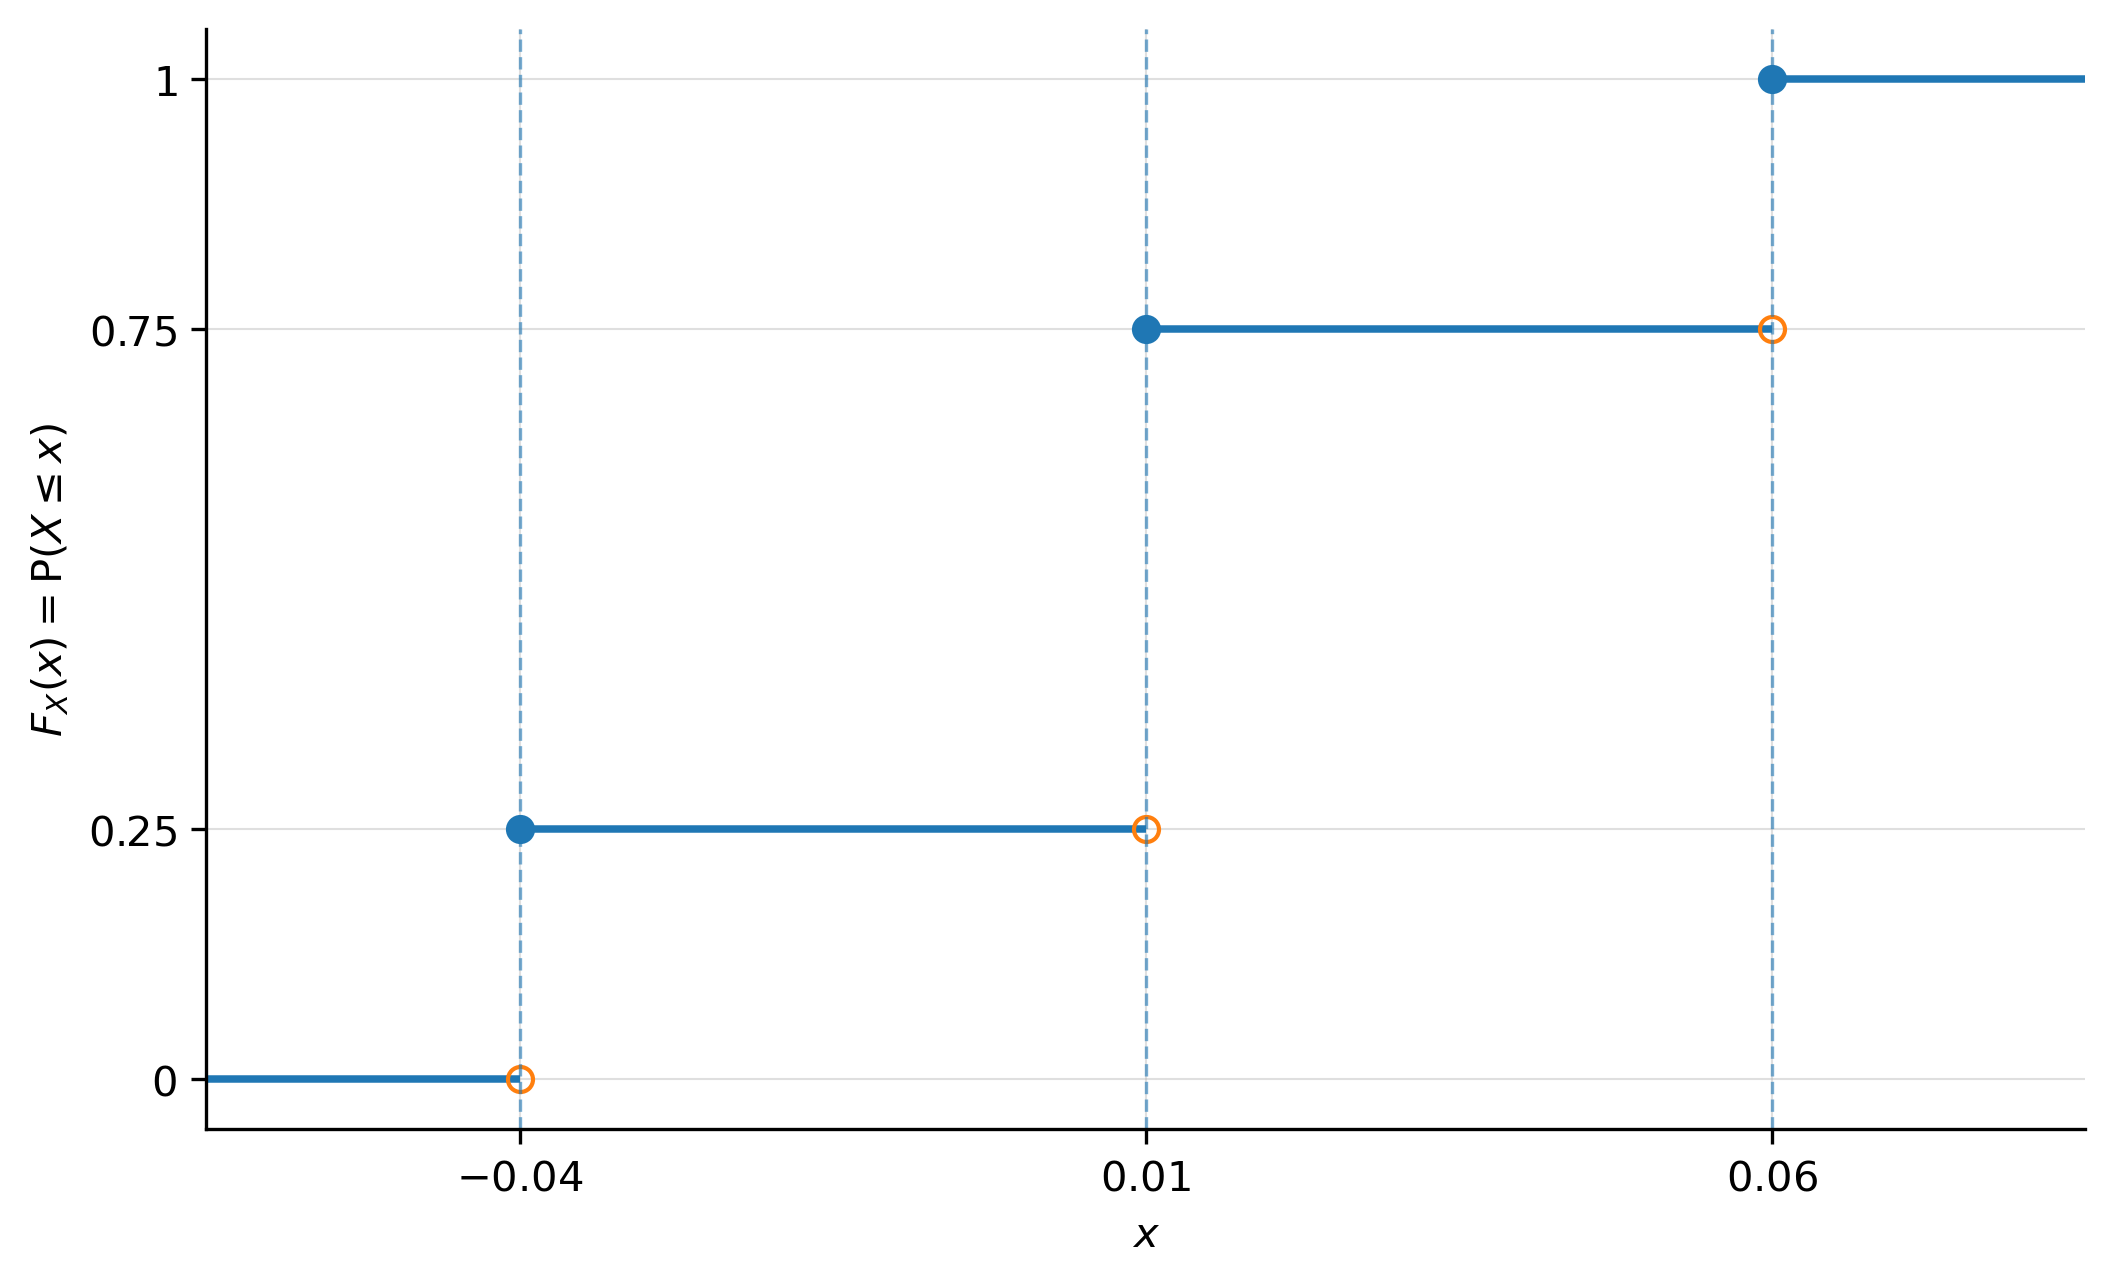
\includegraphics[width=0.78\textwidth]{Cap02_cdf_rendimento_discreto.png}
\end{center}

La continuit\`{a} da destra determina il valore della funzione nei punti di salto.%

%TCIMACRO{\TeXButton{Transition: Box Out}{\transboxout}}%
%BeginExpansion
\transboxout
%EndExpansion%
%TCIMACRO{\TeXButton{EndFrame}{\end{frame}}}%
%BeginExpansion
\end{frame}%
%EndExpansion


%***********************************


\subsection{Variabili casuali continue e densit\`{a}}%

%TCIMACRO{\TeXButton{BeginFrame}{\begin{frame}}}%
%BeginExpansion
\begin{frame}%
%EndExpansion
%

%TCIMACRO{\QTR{frametitle}{Variabili continue e densit\`{a}}}%
%BeginExpansion
\frametitle{Variabili continue e densit\`{a}}%
%EndExpansion


Nel caso continuo, la probabilit\`{a} non \`{e} concentrata sui singoli valori.

\medskip

Una variabile casuale $X$ \`{e} \textbf{assolutamente continua} se esiste una
funzione $f_{X}:\mathbb{R}\to[0,+\infty)$ tale che%

\[
\Prob_{X}(B) = \Prob(X\in B) = \int_{B} f_{X}(x)\,dx, \qquad B\in
\mathcal{B}(\mathbb{R}).
\]


\medskip

$f_{X}$ \`{e} detta \textbf{funzione di densit\`{a}} (di probabilit\`{a}) di
$X$.

\medskip

Condizioni fondamentali:%

\[
f_{X}(x)\geq0, \qquad\int_{-\infty}^{+\infty}f_{X}(x)\,dx=1.
\]
%

%TCIMACRO{\TeXButton{Transition: Box Out}{\transboxout}}%
%BeginExpansion
\transboxout
%EndExpansion%
%TCIMACRO{\TeXButton{EndFrame}{\end{frame}}}%
%BeginExpansion
\end{frame}%
%EndExpansion


%***********************************


\subsection{Probabilit\`{a} come area}%

%TCIMACRO{\TeXButton{BeginFrame}{\begin{frame}}}%
%BeginExpansion
\begin{frame}%
%EndExpansion
%

%TCIMACRO{\QTR{frametitle}{Probabilit\`{a} come area sotto la densit\`{a}}}%
%BeginExpansion
\frametitle{Probabilit\`{a} come area sotto la densit\`{a}}%
%EndExpansion


Per $a<b$, la probabilit\`{a} che $X$ appartenga all'intervallo $(a,b]$ \`{e}%

\[
\Prob(a<X\leq b) = \int_{a}^{b} f_{X}(x)\,dx.
\]


\medskip

Nel caso assolutamente continuo, i singoli punti hanno probabilit\`{a} nulla:%

\[
\Prob(X=x)=0, \qquad x\in\mathbb{R}.
\]


\medskip

Quindi l'inclusione o esclusione degli estremi non modifica la probabilit\`{a}:%

\[
\Prob(a<X<b) = \Prob(a\leq X\leq b) = \int_{a}^{b} f_{X}(x)\,dx.
\]


\medskip

Attenzione: $f_{X}(x)$ non \`{e} una probabilit\`{a}; la probabilit\`{a} \`{e}
l'area sotto la densit\`{a}.%

%TCIMACRO{\TeXButton{Transition: Box Out}{\transboxout}}%
%BeginExpansion
\transboxout
%EndExpansion%
%TCIMACRO{\TeXButton{EndFrame}{\end{frame}}}%
%BeginExpansion
\end{frame}%
%EndExpansion


%***********************************


\subsection{Probabilit\`{a} come area}%

%TCIMACRO{\TeXButton{BeginFrame}{\begin{frame}}}%
%BeginExpansion
\begin{frame}%
%EndExpansion
%

%TCIMACRO{\QTR{frametitle}{Probabilit\`{a} come area sotto la densit\`{a}}}%
%BeginExpansion
\frametitle{Probabilit\`{a} come area sotto la densit\`{a}}%
%EndExpansion


L'area compresa tra $a$ e $b$ rappresenta la probabilit\`{a} che la variabile
casuale $X$ assuma valori in quell'intervallo.

\medskip

\begin{center}
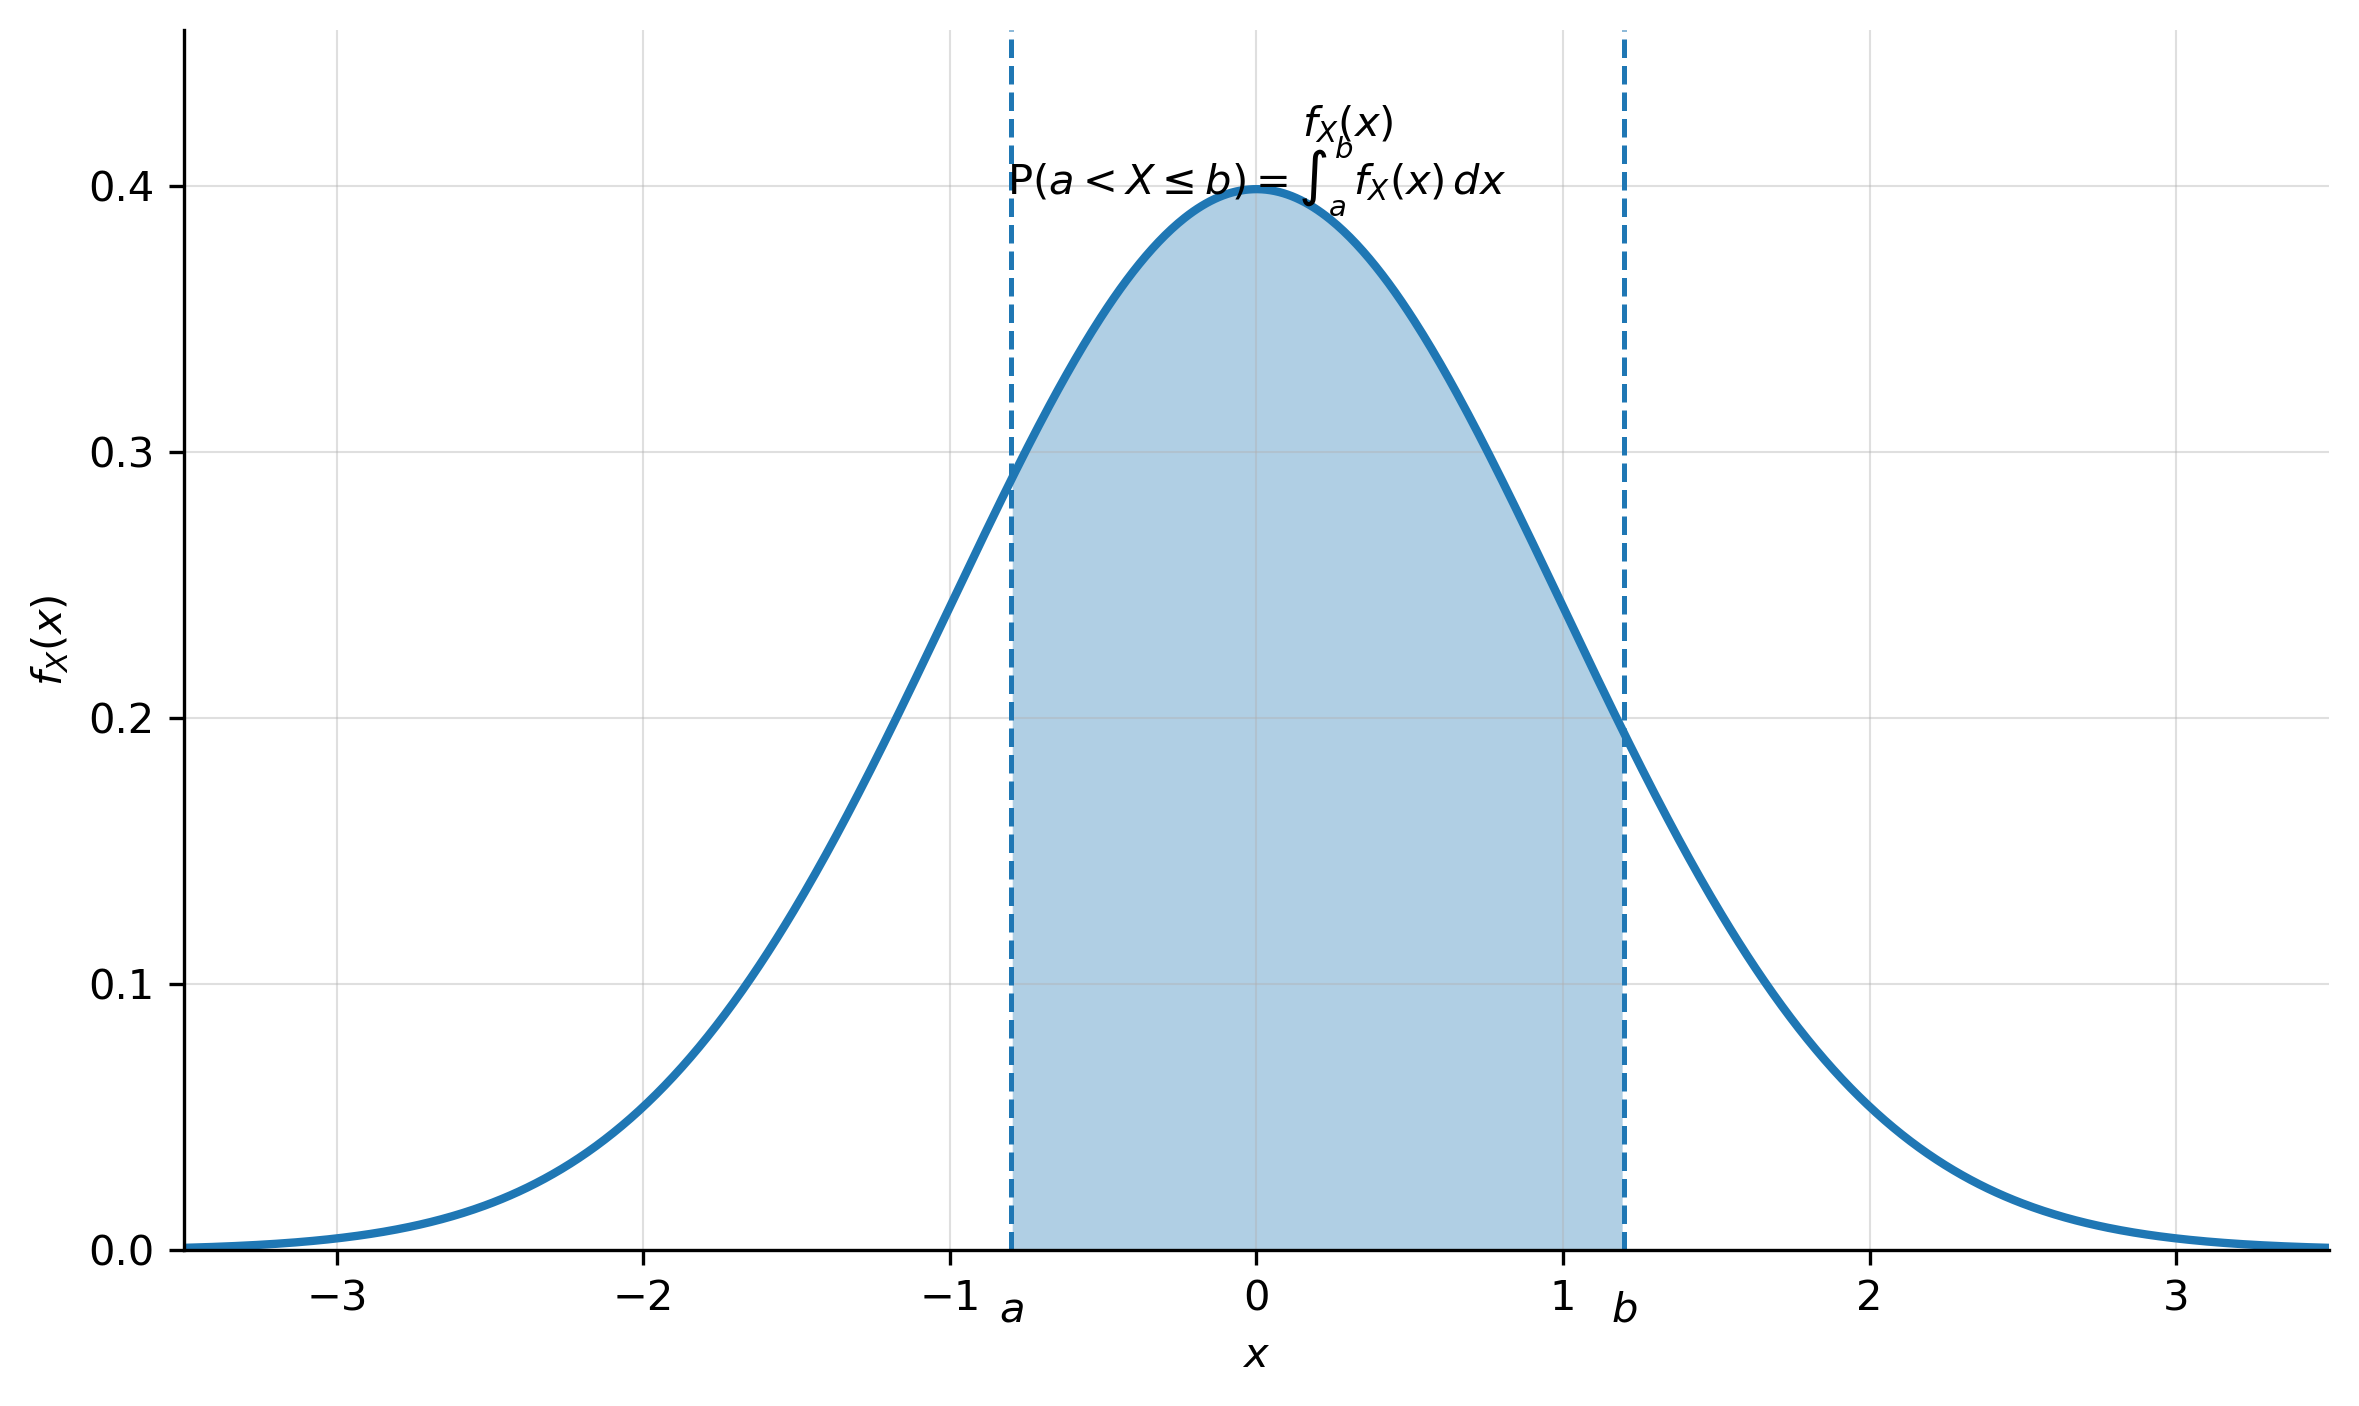
\includegraphics[width=0.82\textwidth]{Cap02_probabilita_area_sotto_densita.png}
\end{center}%

%TCIMACRO{\TeXButton{Transition: Box Out}{\transboxout}}%
%BeginExpansion
\transboxout
%EndExpansion%
%TCIMACRO{\TeXButton{EndFrame}{\end{frame}}}%
%BeginExpansion
\end{frame}%
%EndExpansion


%***********************************


\subsection{Probabilit\`{a} di un punto}%

%TCIMACRO{\TeXButton{BeginFrame}{\begin{frame}}}%
%BeginExpansion
\begin{frame}%
%EndExpansion
%

%TCIMACRO{\QTR{frametitle}{Se l'intervallo si restringe a un punto}}%
%BeginExpansion
\frametitle{Se l'intervallo si restringe a un punto}%
%EndExpansion


Se l'intervallo $[a,b]$ si restringe, l'area sottesa dalla densit\`{a} tende a zero.%

\[
a\leftarrow b \qquad\Longrightarrow\qquad\int_{a}^{a} f_{X}(x)\,dx\to0
\]


\medskip

Quindi, nel caso assolutamente continuo,%

\[
\Prob(X=a)=0.
\]


\medskip

Pi\`{u} in generale,%

\[
\Prob(X=x)=0, \qquad x\in\mathbb{R}.
\]


\medskip

La probabilit\`{a} non \`{e} attribuita ai singoli punti, ma agli intervalli,
cio\`{e} alle aree sotto la densit\`{a}.%

%TCIMACRO{\TeXButton{Transition: Box Out}{\transboxout}}%
%BeginExpansion
\transboxout
%EndExpansion%
%TCIMACRO{\TeXButton{EndFrame}{\end{frame}}}%
%BeginExpansion
\end{frame}%
%EndExpansion


%***********************************


\subsection{Densit\`{a} e funzione di distribuzione}%

%TCIMACRO{\TeXButton{BeginFrame}{\begin{frame}}}%
%BeginExpansion
\begin{frame}%
%EndExpansion
%

%TCIMACRO{\QTR{frametitle}{Densit\`{a} e funzione di distribuzione}}%
%BeginExpansion
\frametitle{Densit\`{a} e funzione di distribuzione}%
%EndExpansion


La funzione di distribuzione si ottiene integrando la densit\`{a}:%

\[
F_{X}(x) = \Prob(X\leq x) = \int_{-\infty}^{x} f_{X}(s)\,ds.
\]


\medskip

Se $F_{X}$ \`{e} derivabile nel punto $x$, allora%

\[
f_{X}(x)=F_{X}^{\prime}(x).
\]


\medskip

Interpretazione locale:%

\[
\Prob\left( x-\frac{\varepsilon}{2}<X\leq x+\frac{\varepsilon}{2}\right)
\simeq\varepsilon f_{X}(x), \qquad\varepsilon\mbox{ piccolo}.
\]


\medskip

La densit\`{a} misura la rapidit\`{a} con cui la probabilit\`{a} si accumula
intorno a un valore.%

%TCIMACRO{\TeXButton{Transition: Box Out}{\transboxout}}%
%BeginExpansion
\transboxout
%EndExpansion%
%TCIMACRO{\TeXButton{EndFrame}{\end{frame}}}%
%BeginExpansion
\end{frame}%
%EndExpansion


%***********************************


\subsection{Esempio uniforme}%

%TCIMACRO{\TeXButton{BeginFrame}{\begin{frame}}}%
%BeginExpansion
\begin{frame}%
%EndExpansion
%

%TCIMACRO{\QTR{frametitle}{Esempio: rendimento uniforme}}%
%BeginExpansion
\frametitle{Esempio: rendimento uniforme}%
%EndExpansion


Sia $R$ un rendimento continuo con densit\`{a} uniforme su $[-0.04,0.06]$:%

\[
f_{R}(r)=
\begin{cases}
10, & -0.04\leq r\leq0.06,\\
0, & \mbox{altrove}.
\end{cases}
\]


\medskip

La densit\`{a} \`{e} costante sull'intervallo dei valori possibili.%

\[
\int_{-\infty}^{+\infty} f_{R}(r)\,dr = \int_{-0.04}^{0.06}10\,dr = 10(0.10) =
1.
\]


\medskip

La normalizzazione conferma che $f_{R}$ \`{e} una densit\`{a} di probabilit\`{a}.%

%TCIMACRO{\TeXButton{Transition: Box Out}{\transboxout}}%
%BeginExpansion
\transboxout
%EndExpansion%
%TCIMACRO{\TeXButton{EndFrame}{\end{frame}}}%
%BeginExpansion
\end{frame}%
%EndExpansion


%***********************************


\subsection{Area di probabilit\`{a} nell'esempio uniforme}%

%TCIMACRO{\TeXButton{BeginFrame}{\begin{frame}}}%
%BeginExpansion
\begin{frame}%
%EndExpansion
%

%TCIMACRO{\QTR{frametitle}{Esempio uniforme: probabilit\`{a} di un
%intervallo}}%
%BeginExpansion
\frametitle{Esempio uniforme: probabilit\`{a} di un intervallo}%
%EndExpansion


L'area evidenziata rappresenta la probabilit\`{a} che il rendimento sia
compreso tra $1\%$ e $5\%$.

\medskip

\begin{center}
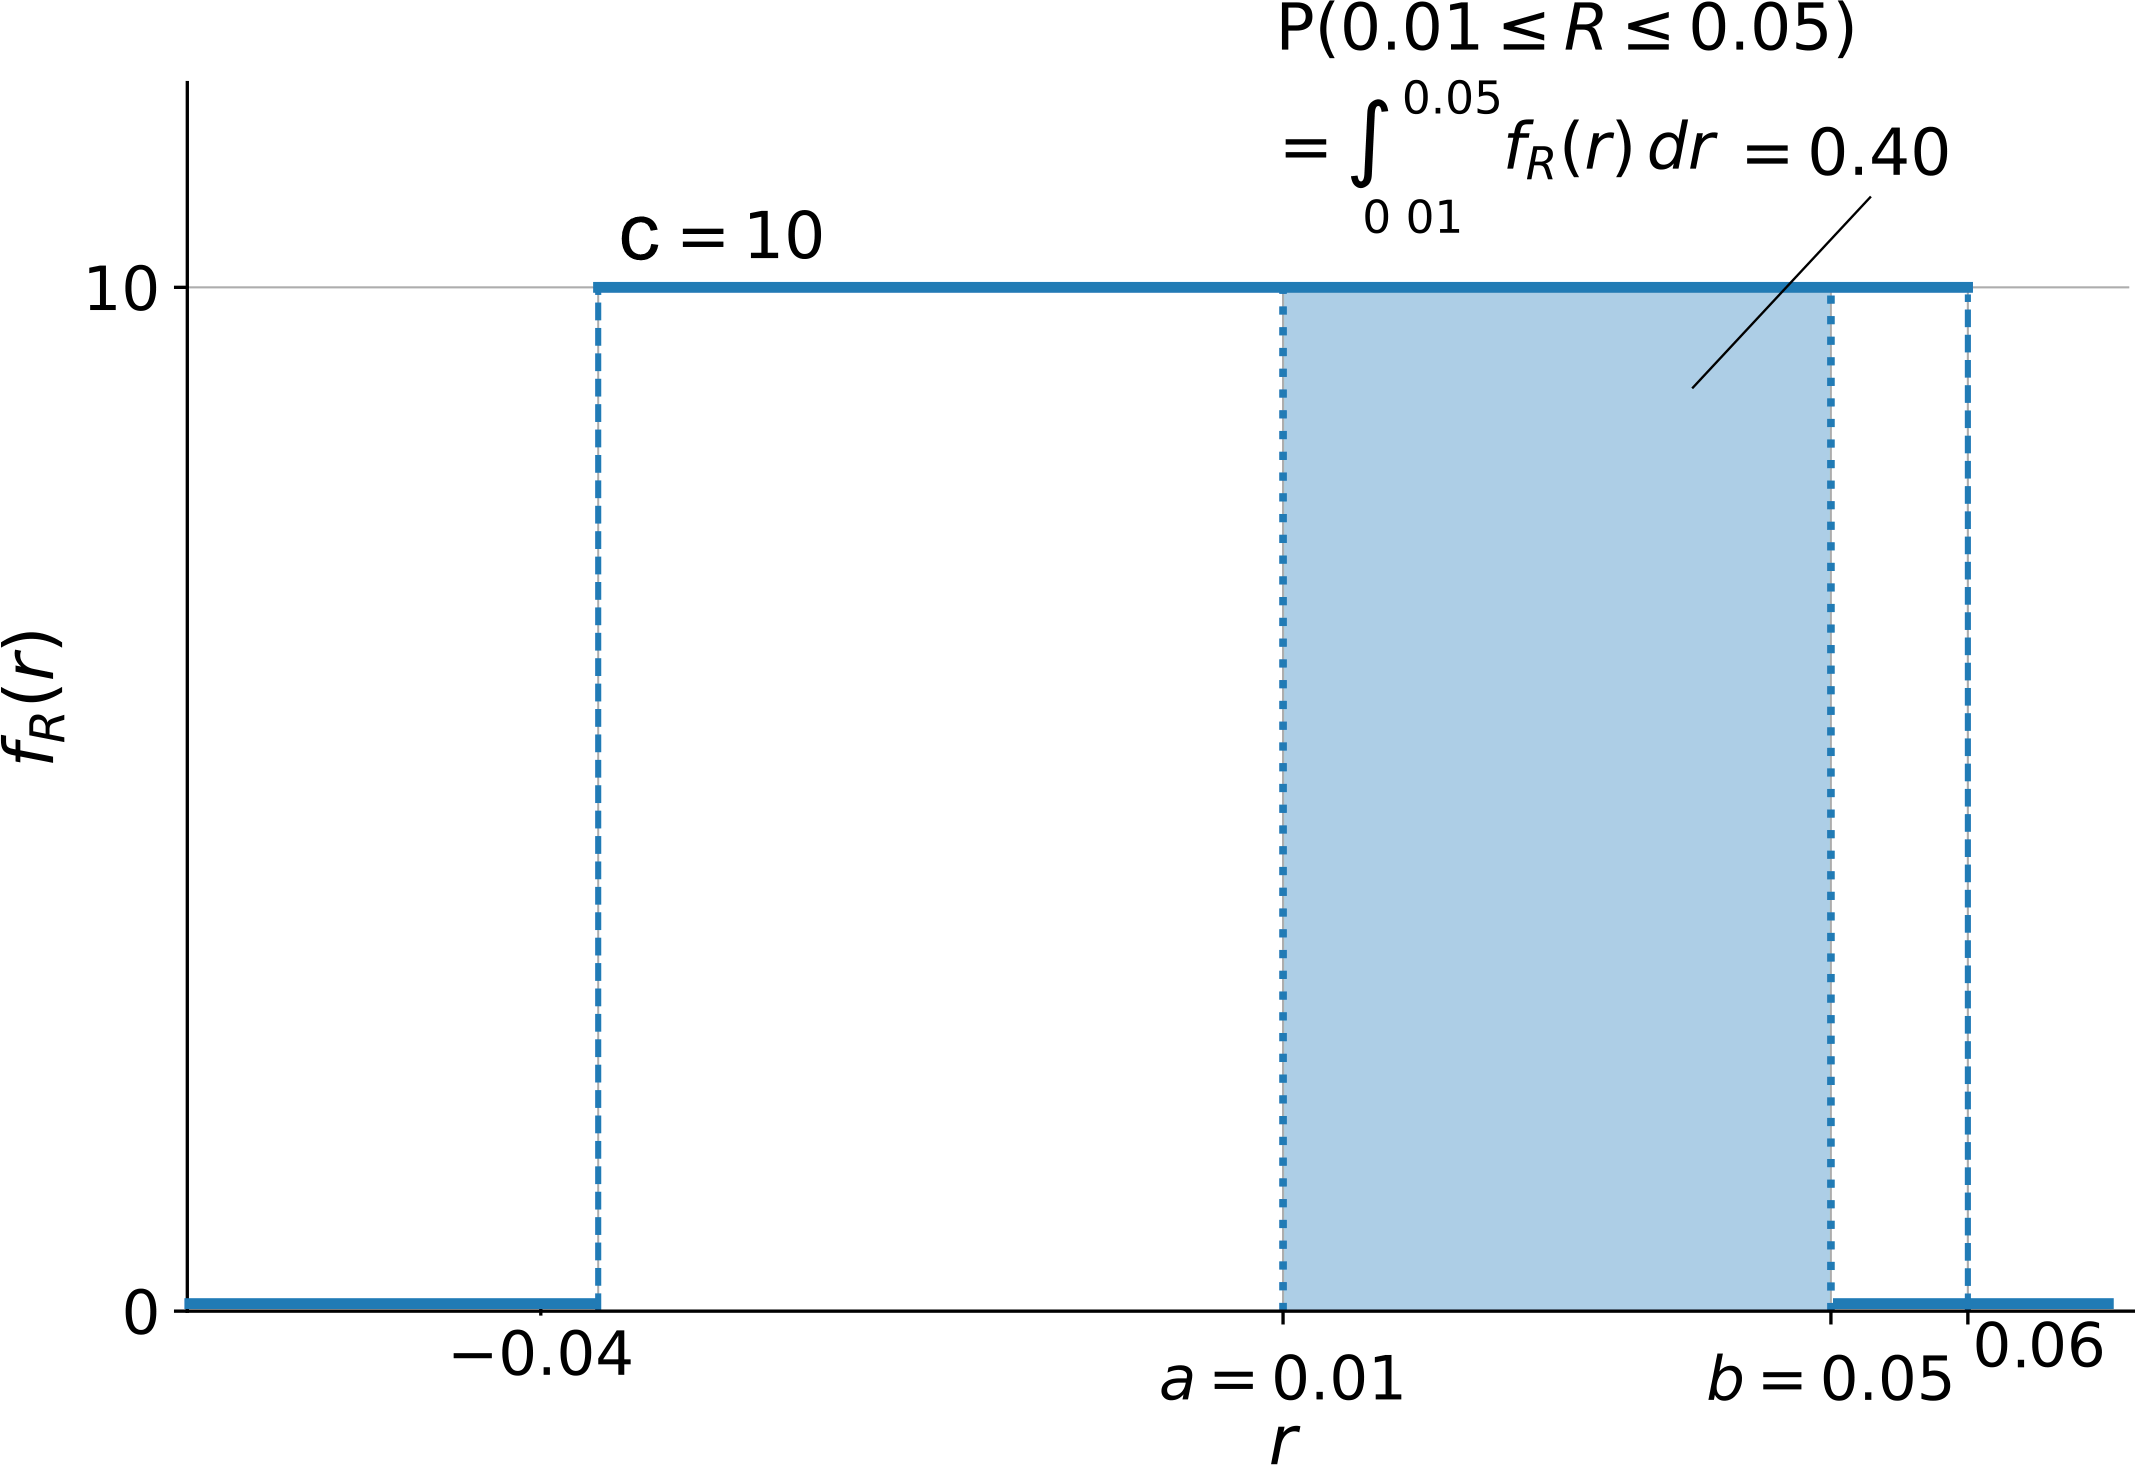
\includegraphics[width=0.78\textwidth]{Cap02_densita_uniforme_rendimento_area_01_05.png}
\end{center}%

%TCIMACRO{\TeXButton{Transition: Box Out}{\transboxout}}%
%BeginExpansion
\transboxout
%EndExpansion%
%TCIMACRO{\TeXButton{EndFrame}{\end{frame}}}%
%BeginExpansion
\end{frame}%
%EndExpansion


%***********************************


\subsection{Probabilit\`{a} di coda}%

%TCIMACRO{\TeXButton{BeginFrame}{\begin{frame}}}%
%BeginExpansion
\begin{frame}%
%EndExpansion
%

%TCIMACRO{\QTR{frametitle}{Probabilit\`{a} di coda}}%
%BeginExpansion
\frametitle{Probabilit\`{a} di coda}%
%EndExpansion


La funzione di distribuzione descrive direttamente le probabilit\`{a} di coda.

\medskip

Coda sinistra:%

\[
\Prob(X\leq x)=F_{X}(x).
\]


\medskip

Coda destra:%

\[
\Prob(X>x)=1-F_{X}(x).
\]


\medskip

Per eventi con disuguaglianza non stretta:%

\[
\Prob(X\geq x)=1-F_{X}(x^{-}).
\]


\medskip

Se $L$ rappresenta una perdita, la probabilit\`{a}%

\[
\Prob(L>\ell)
\]


misura la probabilit\`{a} che la perdita superi la soglia $\ell$.%

%TCIMACRO{\TeXButton{Transition: Box Out}{\transboxout}}%
%BeginExpansion
\transboxout
%EndExpansion%
%TCIMACRO{\TeXButton{EndFrame}{\end{frame}}}%
%BeginExpansion
\end{frame}%
%EndExpansion


%***********************************


\subsection{Quantili}%

%TCIMACRO{\TeXButton{BeginFrame}{\begin{frame}}}%
%BeginExpansion
\begin{frame}%
%EndExpansion
%

%TCIMACRO{\QTR{frametitle}{Quantile di ordine $\alpha$}}%
%BeginExpansion
\frametitle{Quantile di ordine $\alpha$}%
%EndExpansion


Sia $X$ una variabile casuale reale con funzione di distribuzione $F_{X}$.

\medskip

Per $\alpha\in(0,1)$, il quantile di ordine $\alpha$ \`{e}%

\[
q_{\alpha}(X) = \inf\{x\in\mathbb{R}:F_{X}(x)\geq\alpha\}.
\]


\medskip

Il quantile \`{e} la soglia pi\`{u} bassa per cui la probabilit\`{a} cumulata
raggiunge almeno $\alpha$.

\medskip

La definizione tramite infimo \`{e} valida anche quando $F_{X}$ presenta salti.

\medskip

Nel caso discreto, il quantile pu\`{o} coincidere con un punto di salto della
funzione di distribuzione.%

%TCIMACRO{\TeXButton{Transition: Box Out}{\transboxout}}%
%BeginExpansion
\transboxout
%EndExpansion%
%TCIMACRO{\TeXButton{EndFrame}{\end{frame}}}%
%BeginExpansion
\end{frame}%
%EndExpansion


%***********************************


\subsection{Quantili nel caso continuo}%

%TCIMACRO{\TeXButton{BeginFrame}{\begin{frame}}}%
%BeginExpansion
\begin{frame}%
%EndExpansion
%

%TCIMACRO{\QTR{frametitle}{Quantili nel caso continuo}}%
%BeginExpansion
\frametitle{Quantili nel caso continuo}%
%EndExpansion


Se $X$ \`{e} assolutamente continua e $F_{X}$ \`{e} continua e strettamente
crescente nell'intervallo rilevante, il quantile si ottiene risolvendo%

\[
F_{X}(x)=\alpha.
\]


\medskip

In questo caso,%

\[
q_{\alpha}(X)=F_{X}^{-1}(\alpha).
\]


\medskip

Equivalentemente, se $X$ ha densit\`{a} $f_{X}$,%

\[
\int_{-\infty}^{q_{\alpha}(X)} f_{X}(x)\,dx=\alpha.
\]


\medskip

Il quantile individua il punto che lascia a sinistra una probabilit\`{a} pari
ad $\alpha$.%

%TCIMACRO{\TeXButton{Transition: Box Out}{\transboxout}}%
%BeginExpansion
\transboxout
%EndExpansion%
%TCIMACRO{\TeXButton{EndFrame}{\end{frame}}}%
%BeginExpansion
\end{frame}%
%EndExpansion


%***********************************


\subsection{Quantile e rischio di perdita}%

%TCIMACRO{\TeXButton{BeginFrame}{\begin{frame}}}%
%BeginExpansion
\begin{frame}%
%EndExpansion
%

%TCIMACRO{\QTR{frametitle}{Quantile e rischio di perdita}}%
%BeginExpansion
\frametitle{Quantile e rischio di perdita}%
%EndExpansion


Se $L$ rappresenta una perdita, un quantile elevato individua una
\textbf{soglia di rischio}.

\medskip

Per $\alpha$ vicino a $1$,%

\[
q_{\alpha}(L)
\]


\`{e} una soglia tale che la perdita resta sotto quel livello con
probabilit\`{a} almeno $\alpha$. Nel \textbf{caso continuo},%

\[
\Prob(L\leq q_{\alpha}(L))=\alpha,
\]


\medskip

e quindi, perdite di importo maggiore a $q_{\alpha}(L)$ avranno
probabilit\`{a}:
\[
\Prob(L>q_{\alpha}(L))=1-\alpha.
\]


\medskip

Esempio: $q_{0.99}(L)$ \`{e} una soglia superata solo con probabilit\`{a} pari
all'$1\%$.%

%TCIMACRO{\TeXButton{Transition: Box Out}{\transboxout}}%
%BeginExpansion
\transboxout
%EndExpansion%
%TCIMACRO{\TeXButton{EndFrame}{\end{frame}}}%
%BeginExpansion
\end{frame}%
%EndExpansion


%***********************************


\subsection{Quantile normale: esempio}%

%TCIMACRO{\TeXButton{BeginFrame}{\begin{frame}}}%
%BeginExpansion
\begin{frame}%
%EndExpansion
%

%TCIMACRO{\QTR{frametitle}{Coda sinistra e quantile: esempio normale}}%
%BeginExpansion
\frametitle{Coda sinistra e quantile: esempio normale}%
%EndExpansion


Consideriamo un rendimento normale:%

\[
R\sim\mathcal{N}(0.008,0.035^{2}).
\]


\medskip

Il quantile al $5\%$ si ottiene da%

\[
q_{0.05}(R)=\mu+\sigma z_{0.05},
\]


dove%

\[
z_{0.05}\simeq-1.645.
\]


\medskip

Quindi%

\[
q_{0.05}(R) = 0.008+0.035(-1.645) \simeq-0.0496.
\]


\medskip

Interpretazione: il $5\%$ peggiore dei rendimenti si colloca al di sotto di
circa $-4.96\%$.%

%TCIMACRO{\TeXButton{Transition: Box Out}{\transboxout}}%
%BeginExpansion
\transboxout
%EndExpansion%
%TCIMACRO{\TeXButton{EndFrame}{\end{frame}}}%
%BeginExpansion
\end{frame}%
%EndExpansion


%***********************************


\subsection{Quantile normale: grafico}%

%TCIMACRO{\TeXButton{BeginFrame}{\begin{frame}}}%
%BeginExpansion
\begin{frame}%
%EndExpansion
%

%TCIMACRO{\QTR{frametitle}{Coda sinistra e quantile: rappresentazione
%grafica}}%
%BeginExpansion
\frametitle{Coda sinistra e quantile: rappresentazione grafica}%
%EndExpansion


\begin{center}
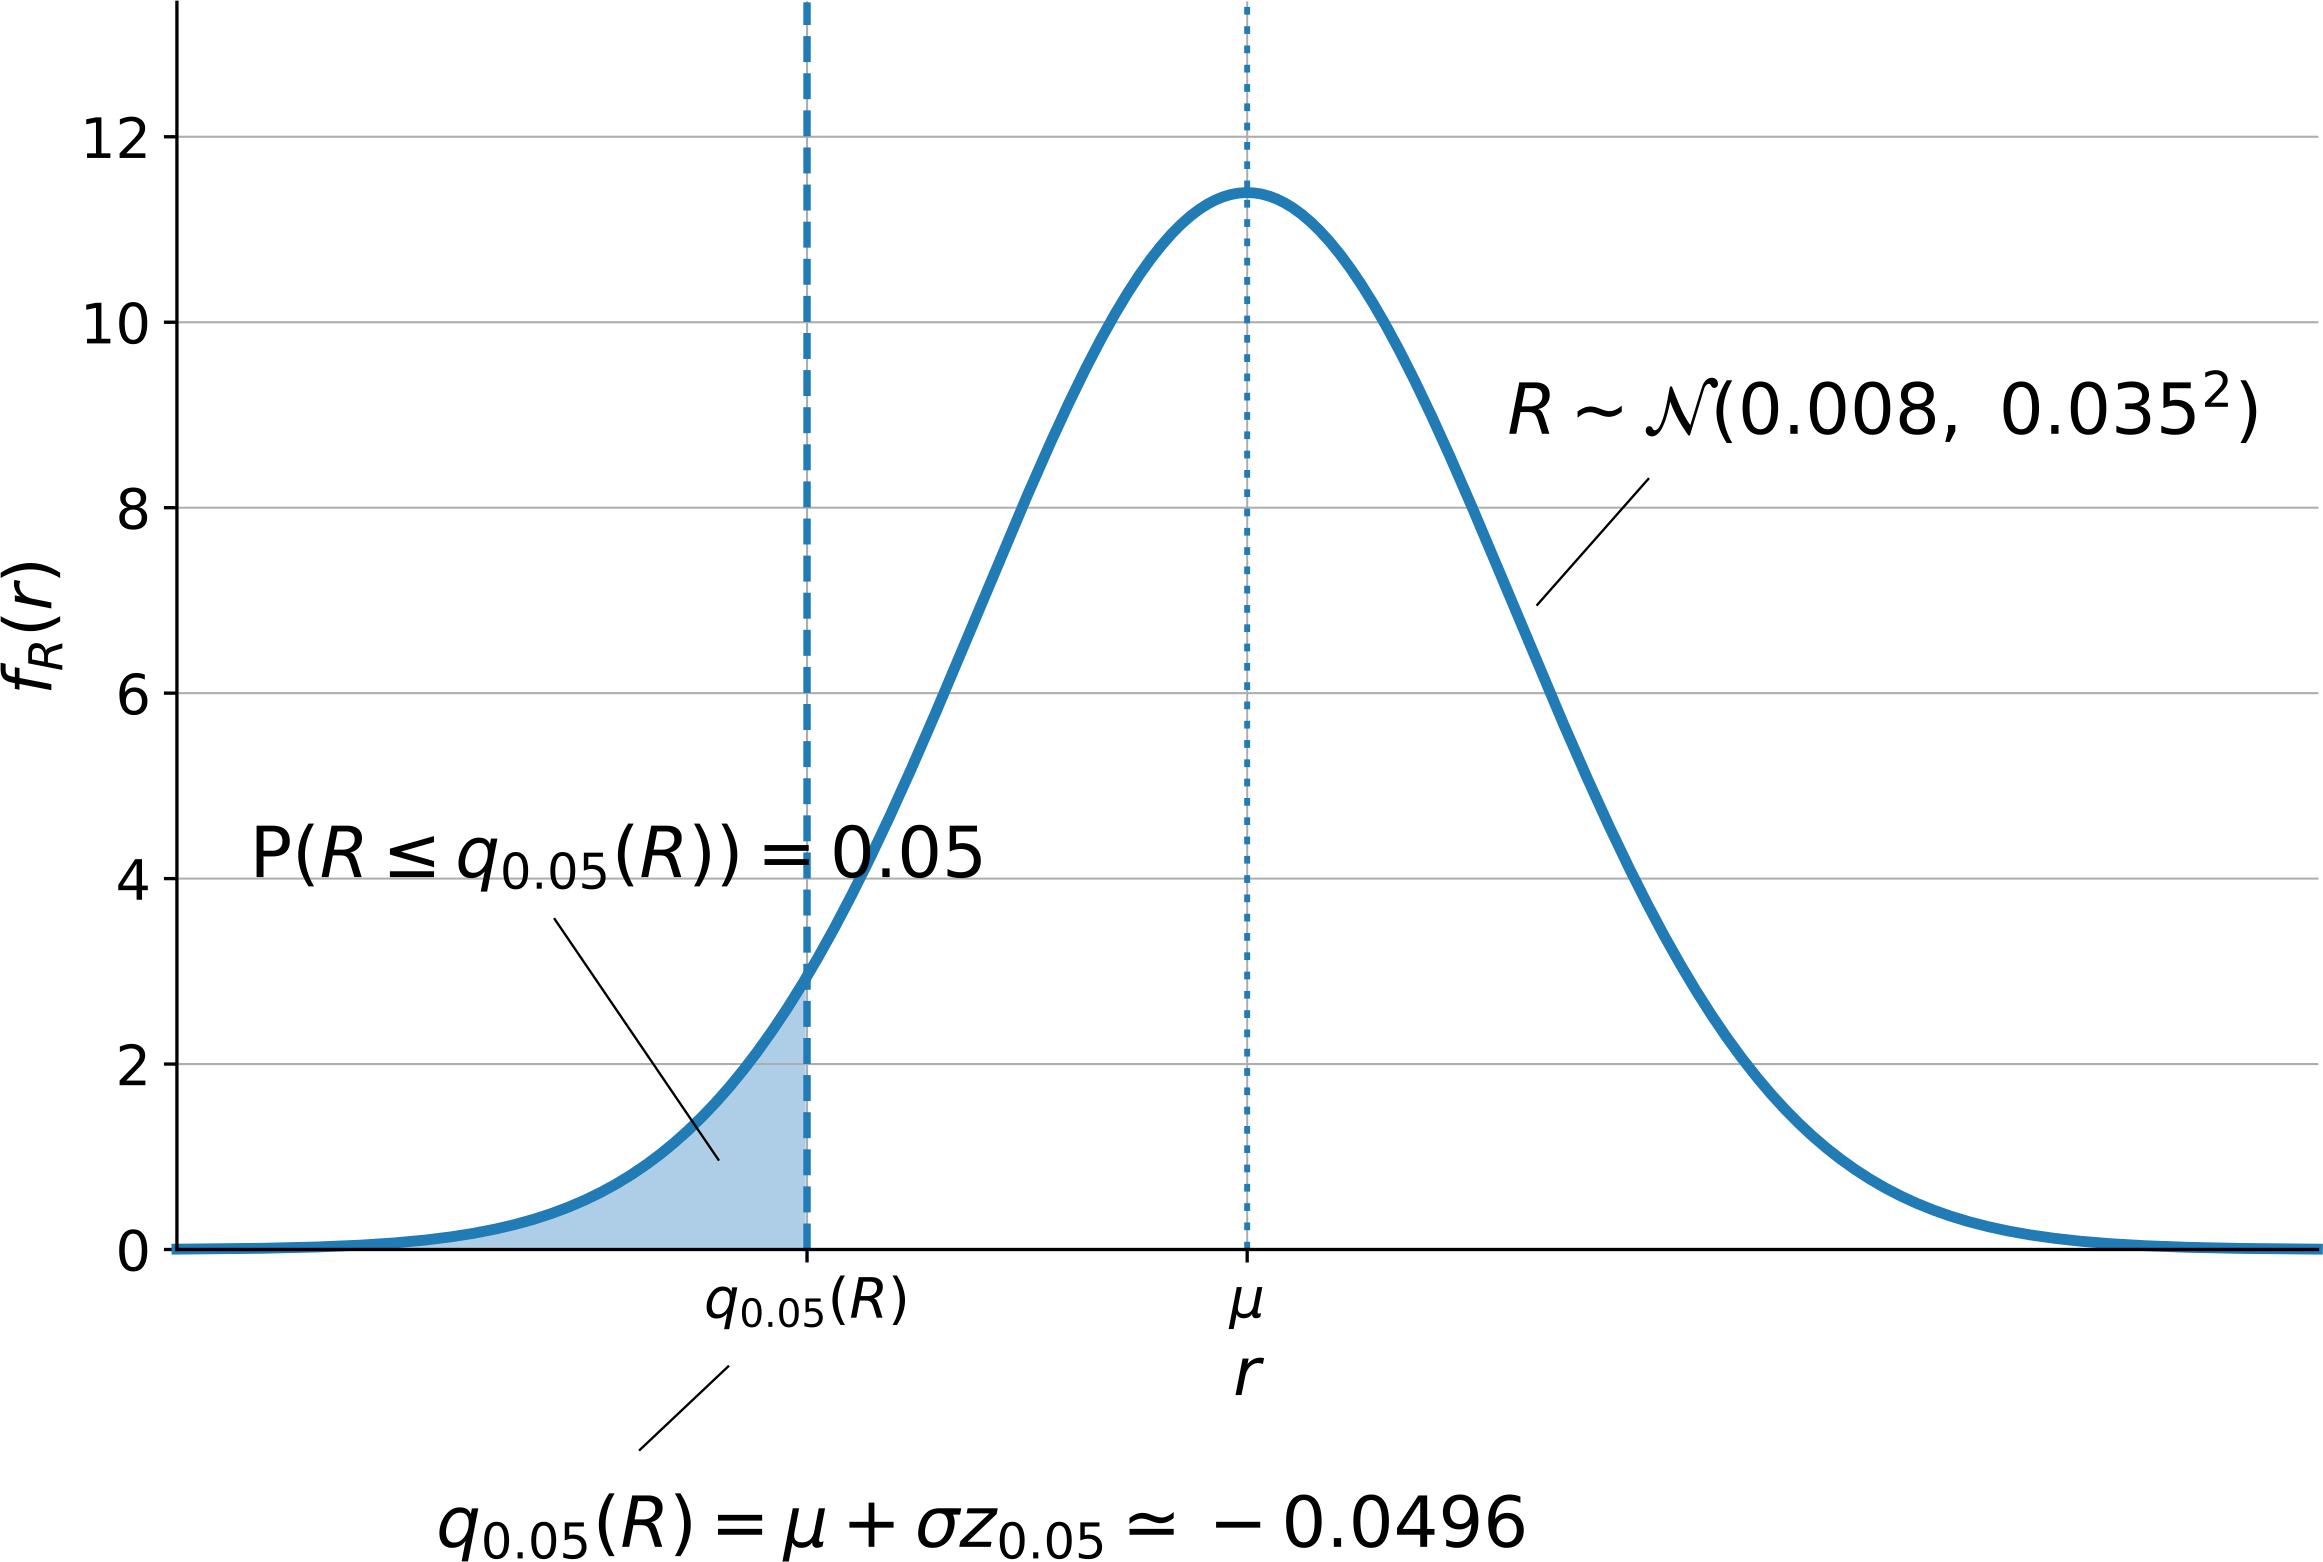
\includegraphics[width=0.80\textwidth]{Cap02_normale_coda_sinistra_quantile_05.png}
\end{center}%

%TCIMACRO{\TeXButton{Transition: Box Out}{\transboxout}}%
%BeginExpansion
\transboxout
%EndExpansion%
%TCIMACRO{\TeXButton{EndFrame}{\end{frame}}}%
%BeginExpansion
\end{frame}%
%EndExpansion


%***********************************


\subsection{Valore atteso}%

%TCIMACRO{\TeXButton{BeginFrame}{\begin{frame}}}%
%BeginExpansion
\begin{frame}%
%EndExpansion
%

%TCIMACRO{\QTR{frametitle}{Valore atteso}}%
%BeginExpansion
\frametitle{Valore atteso}%
%EndExpansion


Il valore atteso sintetizza la posizione media della distribuzione.

\medskip

Caso discreto:%

\[
\E[X] = \sum_{i} x_{i} p_{X}(x_{i}).
\]


\medskip

Caso assolutamente continuo:%

\[
\E[X] = \int_{-\infty}^{+\infty}x f_{X}(x)\,dx.
\]


\medskip

Interpretazione finanziaria:%

\[%
\begin{array}
[c]{rcl}%
\E[R] & : & \mbox{rendimento medio atteso},\\[4pt]%
\E[L] & : & \mbox{perdita attesa},\\[4pt]%
\E[H] & : & \mbox{payoff medio}.
\end{array}
\]
%

%TCIMACRO{\TeXButton{Transition: Box Out}{\transboxout}}%
%BeginExpansion
\transboxout
%EndExpansion%
%TCIMACRO{\TeXButton{EndFrame}{\end{frame}}}%
%BeginExpansion
\end{frame}%
%EndExpansion


%***********************************


\subsection{Linearit\`{a} del valore atteso}%

%TCIMACRO{\TeXButton{BeginFrame}{\begin{frame}}}%
%BeginExpansion
\begin{frame}%
%EndExpansion
%

%TCIMACRO{\QTR{frametitle}{Linearit\`{a} del valore atteso}}%
%BeginExpansion
\frametitle{Linearit\`{a} del valore atteso}%
%EndExpansion


Se $X$ \`{e} integrabile e $a,b\in\mathbb{R}$, allora%

\[
\E[aX+b] = a\E[X]+b.
\]


\medskip

Pi\`{u} in generale, date $X_{i}$, $i=1,\ldots,n$, variabili casuali
integrabili, e dati $a_{i}\in\R$, vale:%

\[
\E\left[ \sum_{i=1}^{n} a_{i}X_{i}\right]  = \sum_{i=1}^{n} a_{i}\E[X_i].
\]


\medskip

Questa propriet\`{a} non richiede indipendenza tra le variabili casuali.

\medskip

Applicazione finanziaria:%

\[
R_{P}=\sum_{i=1}^{n} w_{i} R_{i} \qquad\Longrightarrow\qquad\E[R_P]=\sum
_{i=1}^{n} w_{i}\E[R_i].
\]


\medskip

La linearit\`{a} \`{e} essenziale per rendimenti di portafoglio e
trasformazioni affini.%

%TCIMACRO{\TeXButton{Transition: Box Out}{\transboxout}}%
%BeginExpansion
\transboxout
%EndExpansion%
%TCIMACRO{\TeXButton{EndFrame}{\end{frame}}}%
%BeginExpansion
\end{frame}%
%EndExpansion


%***********************************


\subsection{Valore atteso di funzioni}%

%TCIMACRO{\TeXButton{BeginFrame}{\begin{frame}}}%
%BeginExpansion
\begin{frame}%
%EndExpansion
%

%TCIMACRO{\QTR{frametitle}{Valore atteso di $g(X)$}}%
%BeginExpansion
\frametitle{Valore atteso di $g(X)$}%
%EndExpansion


Spesso l'oggetto finanziario rilevante non \`{e} $X$, ma una funzione di $X$.%

\[
Y=g(X).
\]


\medskip

Caso discreto:%

\[
\E[g(X)] = \sum_{i} g(x_{i})p_{X}(x_{i}).
\]


\medskip

Caso assolutamente continuo:%

\[
\E[g(X)] = \int_{-\infty}^{+\infty} g(x)f_{X}(x)\,dx.
\]
%

%TCIMACRO{\TeXButton{Transition: Box Out}{\transboxout}}%
%BeginExpansion
\transboxout
%EndExpansion%
%TCIMACRO{\TeXButton{EndFrame}{\end{frame}}}%
%BeginExpansion
\end{frame}%
%EndExpansion


%***********************************
%

%TCIMACRO{\TeXButton{BeginFrame}{\begin{frame}}}%
%BeginExpansion
\begin{frame}%
%EndExpansion
%

%TCIMACRO{\QTR{frametitle}{Valore atteso di $g(X)$}}%
%BeginExpansion
\frametitle{Valore atteso di $g(X)$}%
%EndExpansion


Esempio: payoff di una call europea%

\[
H=(S_{T}-K)^{+}.
\]
%

\[
\E[H] = \E[(S_T-K)^+].
\]


\medskip

In generale,%

\[
\E[g(X)]\neq g(\E[X])
\]


quando $g$ non \`{e} lineare.%

%TCIMACRO{\TeXButton{Transition: Box Out}{\transboxout}}%
%BeginExpansion
\transboxout
%EndExpansion%
%TCIMACRO{\TeXButton{EndFrame}{\end{frame}}}%
%BeginExpansion
\end{frame}%
%EndExpansion


%***********************************


\subsection{Variabili indicatrici}%

%TCIMACRO{\TeXButton{BeginFrame}{\begin{frame}}}%
%BeginExpansion
\begin{frame}%
%EndExpansion
%

%TCIMACRO{\QTR{frametitle}{Variabili indicatrici}}%
%BeginExpansion
\frametitle{Variabili indicatrici}%
%EndExpansion


Il valore atteso di una variabile indicatrice coincide con la probabilit\`{a}
dell'evento corrispondente:%

\[
\E[\1_A] = \Prob(A).
\]


\medskip

Esempi finanziari:%

\[
\E[\1_{\{R<0\}}] = \Prob(R<0),
\]
%

\[
\E[\1_{\{L>\ell\}}] = \Prob(L>\ell),
\]
%

\[
\E[\1_{\{S_T>K\}}] = \Prob(S_{T}>K).
\]


\medskip

Le variabili indicatrici trasformano eventi in variabili casuali a valori $0$
e $1$.%

%TCIMACRO{\TeXButton{Transition: Box Out}{\transboxout}}%
%BeginExpansion
\transboxout
%EndExpansion%
%TCIMACRO{\TeXButton{EndFrame}{\end{frame}}}%
%BeginExpansion
\end{frame}%
%EndExpansion


%***********************************


\subsection{Indicatrice dell'evento di rendimento negativo}%

%TCIMACRO{\TeXButton{BeginFrame}{\begin{frame}}}%
%BeginExpansion
\begin{frame}%
%EndExpansion
%

%TCIMACRO{\QTR{frametitle}{Indicatrice dell'evento di rendimento negativo}}%
%BeginExpansion
\frametitle{Indicatrice dell'evento di rendimento negativo}%
%EndExpansion


Sia $r$ uno dei possibili valori della variabile casuale $R$, rendimento di un portafoglio.

\medskip

La funzione indicatrice dell'evento ``rendimento negativo'' \`{e}:%

\[
\1_{\{R<0\}}=
\begin{cases}
1, & \mbox{se } R<0,\\
0, & \mbox{se } R\geq0.
\end{cases}
\]


\medskip

Il suo valore atteso ha una chiara interpretazione:

\medskip%

\[
\E[\1_{\{R<0\}}] = \Prob(R<0).
\]
%

%TCIMACRO{\TeXButton{Transition: Box Out}{\transboxout}}%
%BeginExpansion
\transboxout
%EndExpansion%
%TCIMACRO{\TeXButton{EndFrame}{\end{frame}}}%
%BeginExpansion
\end{frame}%
%EndExpansion


%***********************************


\subsection{Shortfall}%

%TCIMACRO{\TeXButton{BeginFrame}{\begin{frame}}}%
%BeginExpansion
\begin{frame}%
%EndExpansion
%

%TCIMACRO{\QTR{frametitle}{Perdita percentuale rispetto alla soglia zero:
%grafico}}%
%BeginExpansion
\frametitle{Perdita percentuale rispetto alla soglia zero: grafico}%
%EndExpansion


Introduciamo la funzione $g(r)$, perdita percentuale:%

\[
g(r)=(-r)^{+}=-r\,\1_{\{r<0\}}.
\]


\medskip

\begin{center}
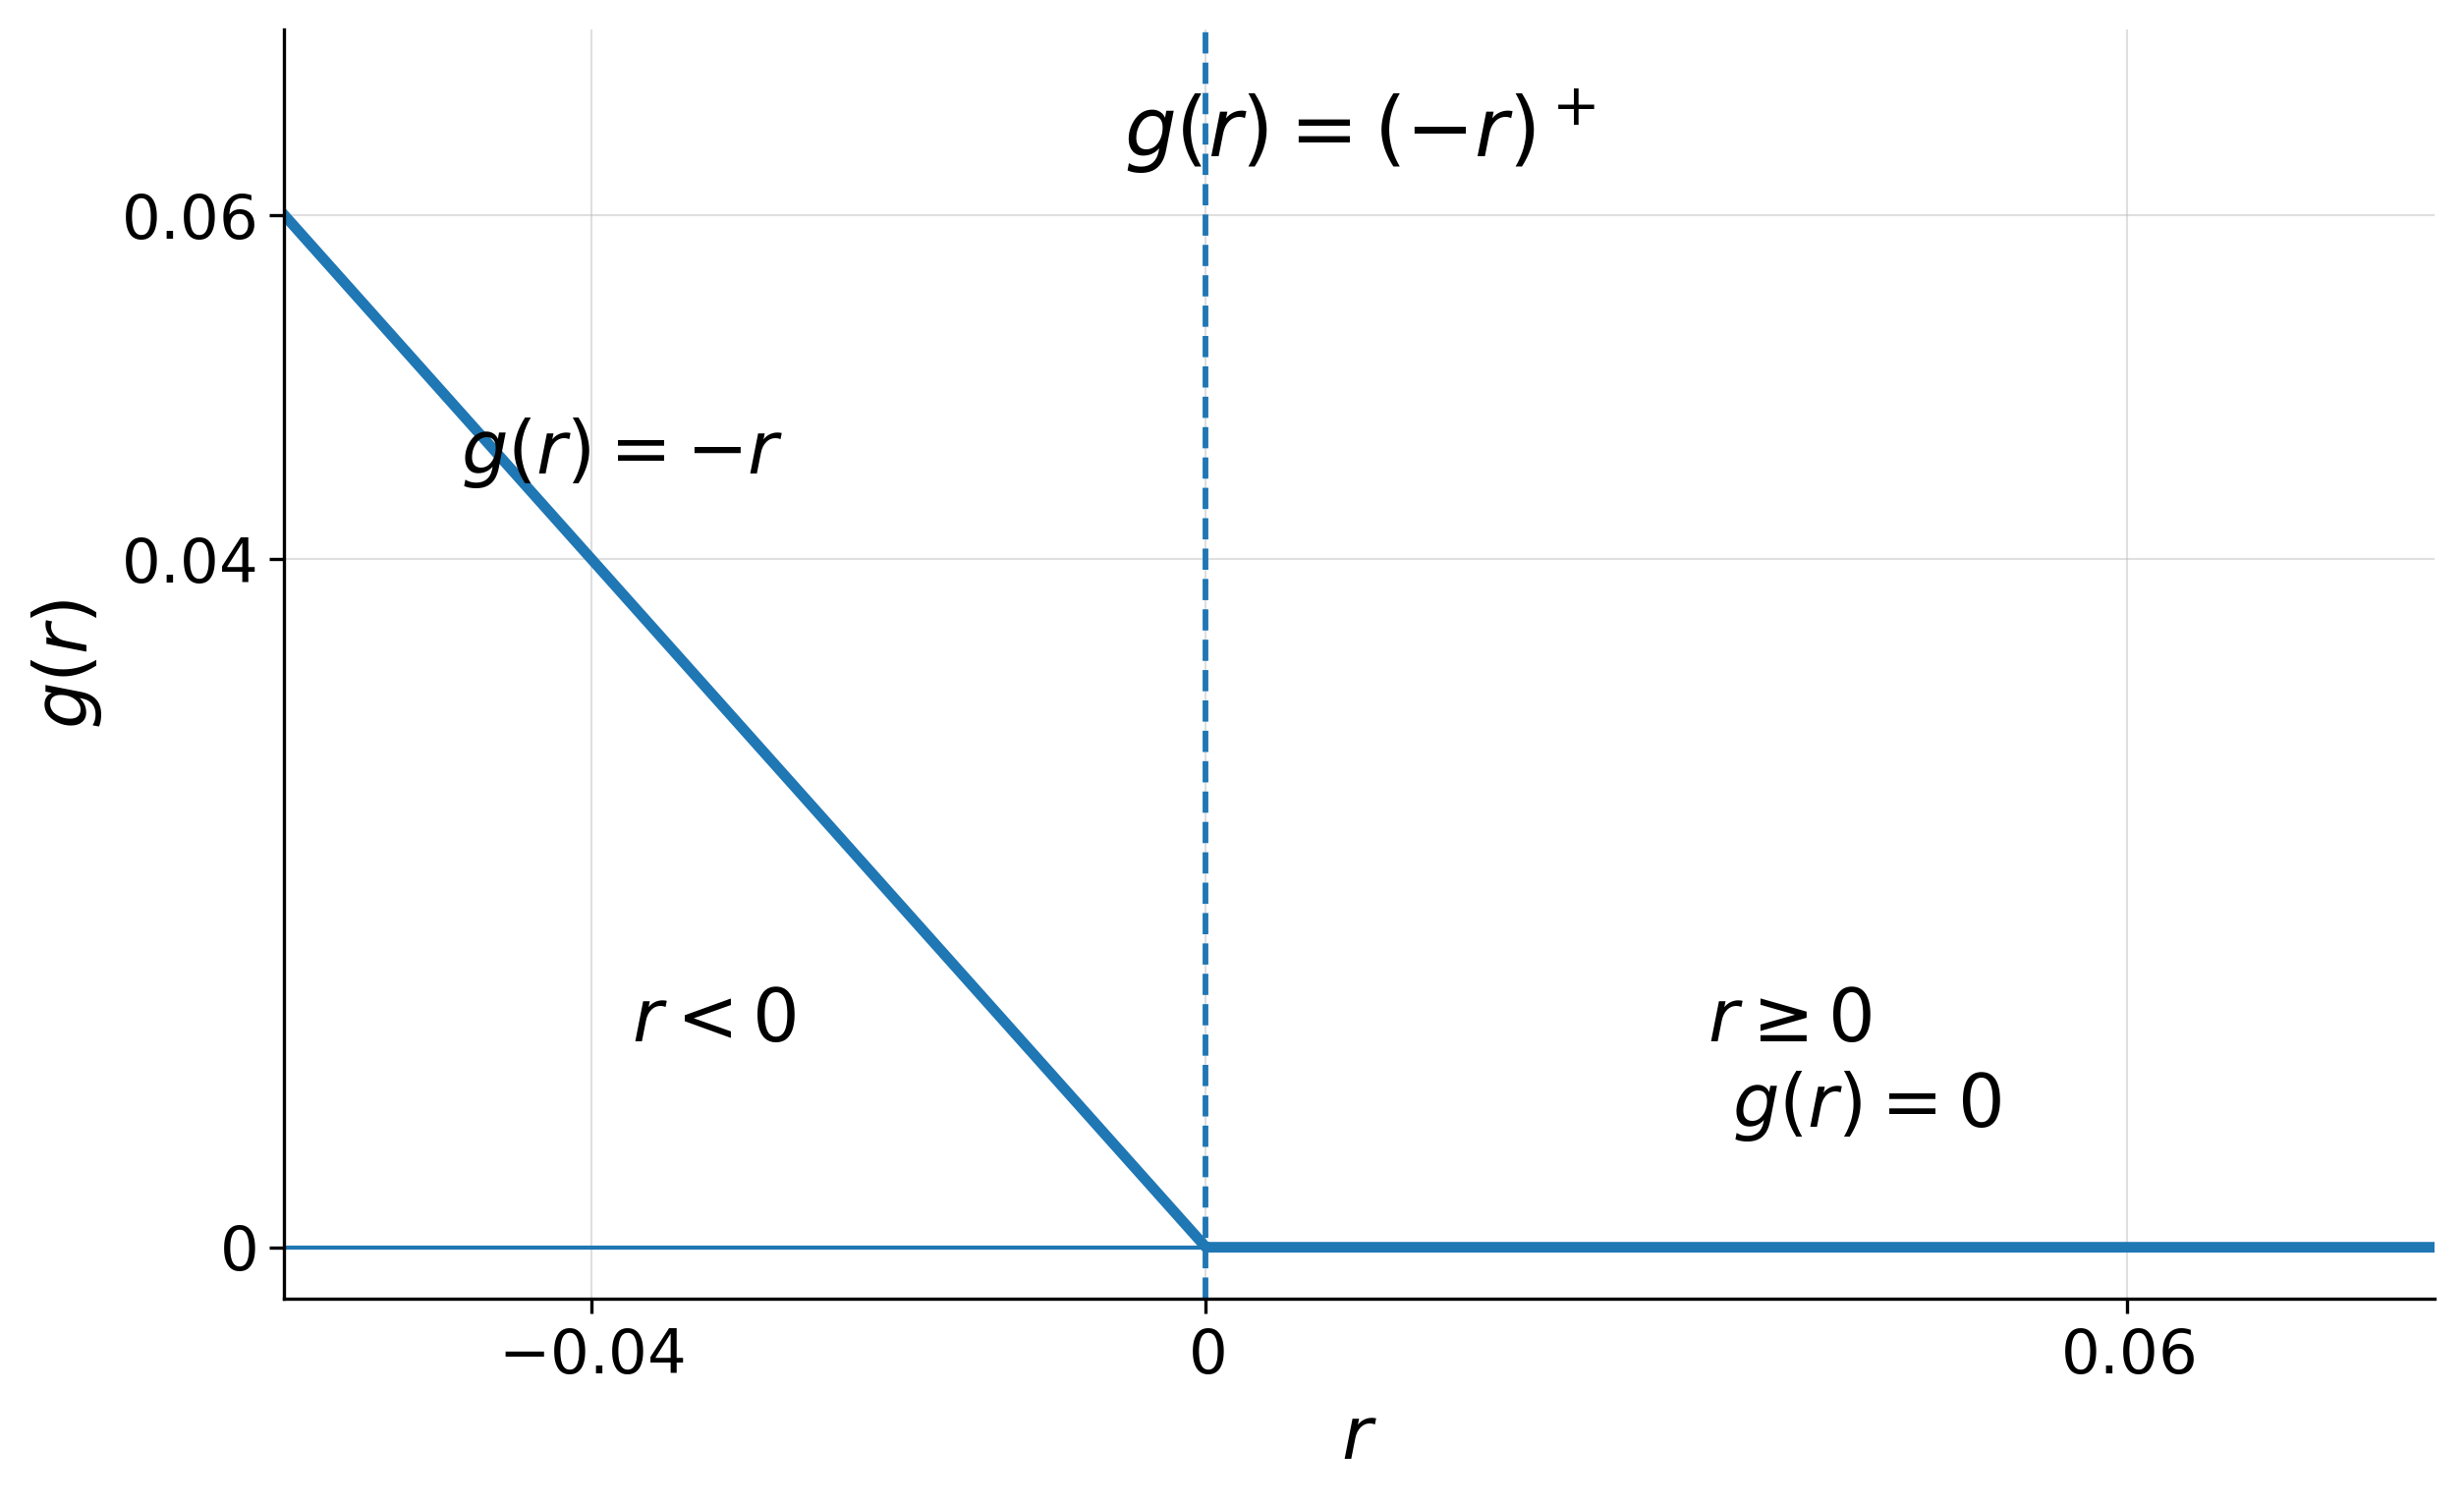
\includegraphics[width=0.80\textwidth]{Cap02_funzione_shortfall_zero.png}
\end{center}%

%TCIMACRO{\TeXButton{Transition: Box Out}{\transboxout}}%
%BeginExpansion
\transboxout
%EndExpansion%
%TCIMACRO{\TeXButton{EndFrame}{\end{frame}}}%
%BeginExpansion
\end{frame}%
%EndExpansion


%***********************************
%

%TCIMACRO{\TeXButton{BeginFrame}{\begin{frame}}}%
%BeginExpansion
\begin{frame}%
%EndExpansion
%

%TCIMACRO{\QTR{frametitle}{Dalla perdita percentuale allo shortfall atteso}}%
%BeginExpansion
\frametitle{Dalla perdita percentuale allo shortfall atteso}%
%EndExpansion


La slide precedente ha definito la perdita percentuale associata ai rendimenti negativi:%

\[
g(r)=(-r)^{+}.
\]


Se $R$ \`{e} il rendimento aleatorio, allora%

\[
g(R)=(-R)^{+}
\]


\`{e} la corrispondente perdita percentuale aleatoria.

\medskip

Il suo valore atteso%

\[
\E[g(R)] = \E[(-R)^+]
\]


misura la perdita percentuale media associata agli scenari di rendimento negativo.

\medskip

Questa quantit\`{a} rappresenta lo \emph{shortfall atteso} rispetto alla
soglia zero.

%\QTR{frametitle}{Shortfall come perdita attesa}


%Un indicatore di interesse finanziario \`{e} lo \emph{shortfall}, inteso come valore atteso della perdita condizionato al verificarsi di un rendimento negativo:


%\[
%\operatorname{SF}
%=
%\mathbb{E}[g(r)\mid r<0]
%=
%\mathbb{E}[-r\mid r<0].
%\]


%Esso rappresenta quindi la perdita percentuale media osservata nei soli scenari sfavorevoli.
%

%TCIMACRO{\TeXButton{Transition: Box Out}{\transboxout}}%
%BeginExpansion
\transboxout
%EndExpansion%
%TCIMACRO{\TeXButton{EndFrame}{\end{frame}}}%
%BeginExpansion
\end{frame}%
%EndExpansion


%***********************************


\subsection{Varianza}%

%TCIMACRO{\TeXButton{BeginFrame}{\begin{frame}}}%
%BeginExpansion
\begin{frame}%
%EndExpansion
%

%TCIMACRO{\QTR{frametitle}{Varianza: dispersione intorno alla media}}%
%BeginExpansion
\frametitle{Varianza: dispersione intorno alla media}%
%EndExpansion


Il valore atteso descrive la posizione media della distribuzione, ma non
misura la dispersione.

\medskip

La varianza di $X$ \`{e}%

\[
\Var(X) = \E\left[ (X-\E[X])^{2}\right] .
\]


\medskip

Nel caso discreto,%

\[
\Var(X) = \sum_{i} (x_{i}-\E[X])^{2}p_{X}(x_{i}).
\]


\medskip

Nel caso assolutamente continuo,%

\[
\Var(X) = \int_{-\infty}^{+\infty}(x-\E[X])^{2}f_{X}(x)\,dx.
\]


\medskip

La varianza misura lo scostamento quadratico medio dal valore atteso.%

%TCIMACRO{\TeXButton{Transition: Box Out}{\transboxout}}%
%BeginExpansion
\transboxout
%EndExpansion%
%TCIMACRO{\TeXButton{EndFrame}{\end{frame}}}%
%BeginExpansion
\end{frame}%
%EndExpansion


%***********************************


\subsection{Formula operativa e deviazione standard}%

%TCIMACRO{\TeXButton{BeginFrame}{\begin{frame}}}%
%BeginExpansion
\begin{frame}%
%EndExpansion
%

%TCIMACRO{\QTR{frametitle}{Formula operativa e deviazione standard}}%
%BeginExpansion
\frametitle{Formula operativa e deviazione standard}%
%EndExpansion


Una formula utile nei calcoli \`{e}%

\[
\Var(X) = \E[X^2]-(\E[X])^{2}.
\]


\medskip

La deviazione standard \`{e}%

\[
\sigma_{X} = \sqrt{\Var(X)}.
\]


\medskip%

\[%
\begin{array}
[c]{rcl}%
\Var(X) & : & \mbox{dispersione quadratica},\\[4pt]%
\sigma_{X} & : & \mbox{dispersione nella stessa unit\`{a} di } X.
\end{array}
\]


\medskip

Se $a$ e $b$ sono costanti reali,%

\[
\Var(aX+b)=a^{2}\Var(X),
\]
%

\[
\sigma_{aX+b}=|a|\sigma_{X}.
\]
%

%TCIMACRO{\TeXButton{Transition: Box Out}{\transboxout}}%
%BeginExpansion
\transboxout
%EndExpansion%
%TCIMACRO{\TeXButton{EndFrame}{\end{frame}}}%
%BeginExpansion
\end{frame}%
%EndExpansion


%***********************************


\subsection{Momenti centrali}%

%TCIMACRO{\TeXButton{BeginFrame}{\begin{frame}}}%
%BeginExpansion
\begin{frame}%
%EndExpansion
%

%TCIMACRO{\QTR{frametitle}{Momenti centrali e forma della distribuzione}}%
%BeginExpansion
\frametitle{Momenti centrali e forma della distribuzione}%
%EndExpansion


I momenti centrali descrivono caratteristiche della distribuzione intorno alla media.%

\[
\E[(X-\E[X])^m].
\]


\medskip

Casi principali:%

\[%
\begin{array}
[c]{rcl}%
m=2 & : & \Var(X),\\[4pt]%
m=3 & : & \mbox{asimmetria},\\[4pt]%
m=4 & : & \mbox{peso delle code}.
\end{array}
\]
%

%TCIMACRO{\TeXButton{Transition: Box Out}{\transboxout}}%
%BeginExpansion
\transboxout
%EndExpansion%
%TCIMACRO{\TeXButton{EndFrame}{\end{frame}}}%
%BeginExpansion
\end{frame}%
%EndExpansion


%***********************************


\subsection{Distribuzioni discrete fondamentali}%

%TCIMACRO{\TeXButton{BeginFrame}{\begin{frame}}}%
%BeginExpansion
\begin{frame}%
%EndExpansion
%

%TCIMACRO{\QTR{frametitle}{Distribuzioni discrete fondamentali}}%
%BeginExpansion
\frametitle{Distribuzioni discrete fondamentali}%
%EndExpansion
%

\[%
\begin{array}
[c]{rcl}%
X\sim\operatorname{Bernoulli}(p) & : &
\mbox{evento binario: successo/insuccesso},\\[6pt]%
X\sim\operatorname{Bin}(n,p) & : & \mbox{numero di successi in } n
\mbox{ prove},\\[6pt]%
X\sim\operatorname{Poisson}(\lambda) & : & \mbox{conteggio di eventi rari}.
\end{array}
\]


\medskip%

\[%
\begin{array}
[c]{rcl}%
\operatorname{Bernoulli}(p) & : &
\mbox{default/non default; superamento soglia},\\[6pt]%
\operatorname{Bin}(n,p) & : &
\mbox{numero di rialzi; numero di default},\\[6pt]%
\operatorname{Poisson}(\lambda) & : & \mbox{shock di mercato; eventi rari}.
\end{array}
\]


\medskip

Nel caso discreto, la distribuzione \`{e} descritta dalla funzione di
probabilit\`{a} $p_{X}(x)=\Prob(X=x)$.%

%TCIMACRO{\TeXButton{Transition: Box Out}{\transboxout}}%
%BeginExpansion
\transboxout
%EndExpansion%
%TCIMACRO{\TeXButton{EndFrame}{\end{frame}}}%
%BeginExpansion
\end{frame}%
%EndExpansion


%***********************************


\subsection{Distribuzioni continue fondamentali}%

%TCIMACRO{\TeXButton{BeginFrame}{\begin{frame}}}%
%BeginExpansion
\begin{frame}%
%EndExpansion
%

%TCIMACRO{\QTR{frametitle}{Distribuzioni continue fondamentali}}%
%BeginExpansion
\frametitle{Distribuzioni continue fondamentali}%
%EndExpansion
%

\[%
\begin{array}
[c]{rcl}%
X\sim U[a,b] & : & \mbox{densit\`{a} costante su un intervallo},\\[6pt]%
X\sim\mathcal{N}(\mu,\sigma^{2}) & : &
\mbox{variabile reale simmetrica intorno a } \mu,\\[6pt]%
S\sim\operatorname{Lognormal}(\mu,\sigma^{2}) & : &
\mbox{variabile positiva e asimmetrica}.
\end{array}
\]


\medskip%

\[%
\begin{array}
[c]{rcl}%
U[a,b] & : & \mbox{modello continuo elementare; simulazione},\\[6pt]%
\mathcal{N}(\mu,\sigma^{2}) & : &
\mbox{rendimenti e variazioni di valore},\\[6pt]%
\operatorname{Lognormal}(\mu,\sigma^{2}) & : &
\mbox{prezzi positivi; fattori di crescita}.
\end{array}
\]


\medskip

Nel caso assolutamente continuo, la distribuzione \`{e} descritta dalla
densit\`{a} $f_{X}$ e dalle aree sotto $f_{X}$.%

%TCIMACRO{\TeXButton{Transition: Box Out}{\transboxout}}%
%BeginExpansion
\transboxout
%EndExpansion%
%TCIMACRO{\TeXButton{EndFrame}{\end{frame}}}%
%BeginExpansion
\end{frame}%
%EndExpansion


%***********************************


\subsection{Scelta della distribuzione}%

%TCIMACRO{\TeXButton{BeginFrame}{\begin{frame}}}%
%BeginExpansion
\begin{frame}%
%EndExpansion
%

%TCIMACRO{\QTR{frametitle}{Che cosa incorpora una distribuzione}}%
%BeginExpansion
\frametitle{Che cosa incorpora una distribuzione}%
%EndExpansion


La scelta di una famiglia distributiva non \`{e} solo tecnica: incorpora
ipotesi sulla grandezza aleatoria.

\medskip%

\[%
\begin{array}
[c]{rcl}%
\mbox{supporto} & : & \mbox{quali valori sono possibili},\\[5pt]%
\mbox{forma} & : & \mbox{simmetria, asimmetria, concentrazione},\\[5pt]%
\mbox{dispersione} & : &
\mbox{variabilit\`{a} intorno al valore medio},\\[5pt]%
\mbox{code} & : & \mbox{probabilit\`{a} di valori estremi}.
\end{array}
\]


\medskip

Esempi:%

\[%
\begin{array}
[c]{rcl}%
\mbox{Bernoulli} & : & \mbox{evento s\`{i}/no},\\[4pt]%
\mbox{Binomiale} & : & \mbox{conteggio su prove ripetute},\\[4pt]%
\mbox{Normale} & : & \mbox{variabile reale simmetrica},\\[4pt]%
\mbox{Lognormale} & : & \mbox{grandezza strettamente positiva}.
\end{array}
\]
%

%TCIMACRO{\TeXButton{Transition: Box Out}{\transboxout}}%
%BeginExpansion
\transboxout
%EndExpansion%
%TCIMACRO{\TeXButton{EndFrame}{\end{frame}}}%
%BeginExpansion
\end{frame}%
%EndExpansion


%***********************************


\subsection{Esercizio integrato: rendimento discreto}%

%TCIMACRO{\TeXButton{BeginFrame}{\begin{frame}}}%
%BeginExpansion
\begin{frame}%
%EndExpansion
%

%TCIMACRO{\QTR{frametitle}{Esercizio 1: rendimento discreto asimmetrico}}%
%BeginExpansion
\frametitle{Esercizio 1: rendimento discreto asimmetrico}%
%EndExpansion


Il rendimento $X$ di un portafoglio ha distribuzione%

\[%
\begin{array}
[c]{c|ccccc}%
x & -0.08 & -0.03 & 0.01 & 0.04 & 0.10\\\hline
p_{X}(x) & 0.08 & 0.22 & 0.35 & 0.25 & 0.10
\end{array}
\]


Calcolare:%

\[
F_{X}(x), \qquad\E[X], \qquad\Var(X), \qquad\sigma_{X}.
\]


\medskip

Determinare inoltre:%

\[
\Prob(X<0), \qquad q_{0.05}(X), \qquad q_{0.95}(X).
\]


\medskip

Interpretare i risultati in termini di rendimento atteso, dispersione e
rischio di perdita.%

%TCIMACRO{\TeXButton{Transition: Box Out}{\transboxout}}%
%BeginExpansion
\transboxout
%EndExpansion%
%TCIMACRO{\TeXButton{EndFrame}{\end{frame}}}%
%BeginExpansion
\end{frame}%
%EndExpansion


%***********************************


\subsection{Esercizio integrato: payoff binomiale}%

%TCIMACRO{\TeXButton{BeginFrame}{\begin{frame}}}%
%BeginExpansion
\begin{frame}%
%EndExpansion
%

%TCIMACRO{\QTR{frametitle}{Esercizio 2: payoff binomiale di una call}}%
%BeginExpansion
\frametitle{Esercizio 2: payoff binomiale di una call}%
%EndExpansion


Un titolo ha prezzo iniziale $S_{0}=100$. In ciascuno di tre periodi pu\`{o}
salire di un fattore $u=1.12$ oppure scendere di un fattore $d=0.94$.

\medskip

La probabilit\`{a} di rialzo \`{e} $p=0.55$. Sia $N$ il numero di rialzi:%

\[
N\sim\operatorname{Bin}(3,0.55).
\]


Il prezzo finale \`{e}%

\[
S_{T}(N)=S_{0}u^{N} d^{3-N}.
\]


\medskip

Per una call europea con strike $K=105$,%

\[
H=(S_{T}-K)^{+}.
\]


Calcolare la distribuzione di $N$, i valori $S_{T}(k)$, i payoff $H(k)$ e%

\[
\E[H].
\]
%

%TCIMACRO{\TeXButton{Transition: Box Out}{\transboxout}}%
%BeginExpansion
\transboxout
%EndExpansion%
%TCIMACRO{\TeXButton{EndFrame}{\end{frame}}}%
%BeginExpansion
\end{frame}%
%EndExpansion


%***********************************


\subsection{Esercizio integrato: rendimento normale}%

%TCIMACRO{\TeXButton{BeginFrame}{\begin{frame}}}%
%BeginExpansion
\begin{frame}%
%EndExpansion
%

%TCIMACRO{\QTR{frametitle}{Esercizio 3: rendimento normale e quantile di
%perdita}}%
%BeginExpansion
\frametitle{Esercizio 3: rendimento normale e quantile di perdita}%
%EndExpansion


Il rendimento $R$ di un portafoglio ha distribuzione normale%

\[
R\sim\mathcal{N}(0.008,0.035^{2}).
\]


Calcolare la probabilit\`{a} di rendimento negativo:%

\[
\Prob(R<0).
\]


\medskip

Calcolare il quantile al $5\%$ del rendimento:%

\[
q_{0.05}(R).
\]


\medskip

Definendo la perdita come%

\[
L=-R,
\]


calcolare il quantile al $95\%$ della perdita:%

\[
q_{0.95}(L).
\]


\medskip

Interpretare $q_{0.95}(L)$ come soglia di perdita superata con probabilit\`{a}
pari al $5\%$.%

%TCIMACRO{\TeXButton{Transition: Box Out}{\transboxout}}%
%BeginExpansion
\transboxout
%EndExpansion%
%TCIMACRO{\TeXButton{EndFrame}{\end{frame}}}%
%BeginExpansion
\end{frame}%
%EndExpansion


%***********************************


\subsection{Sintesi concettuale}%

%TCIMACRO{\TeXButton{BeginFrame}{\begin{frame}}}%
%BeginExpansion
\begin{frame}%
%EndExpansion
%

%TCIMACRO{\QTR{frametitle}{Sintesi della lezione}}%
%BeginExpansion
\frametitle{Sintesi della lezione}%
%EndExpansion


Abbiamo trasformato il linguaggio degli eventi in strumenti quantitativi per
rendimenti, perdite e payoff.

\medskip%

\[
(\Omega,\F,\Prob) \quad\longrightarrow\quad X \quad\longrightarrow
\quad\Prob_{X},\ F_{X},\ p_{X},\ f_{X}
\]


\medskip%

\[%
\begin{array}
[c]{rcl}%
(\Omega,\F,\Prob) & : & \mbox{scenari, eventi e probabilit\`{a}},\\[5pt]%
X & : & \mbox{grandezza finanziaria aleatoria},\\[5pt]%
\Prob_{X},\ F_{X},\ p_{X},\ f_{X} & : &
\mbox{descrizione probabilistica dei valori di } X.
\end{array}
\]


\medskip

Idea da trattenere: la distribuzione di $X$ \`{e} il ponte tra scenari incerti
e valori finanziari misurabili.%

%TCIMACRO{\TeXButton{Transition: Box Out}{\transboxout}}%
%BeginExpansion
\transboxout
%EndExpansion%
%TCIMACRO{\TeXButton{EndFrame}{\end{frame}}}%
%BeginExpansion
\end{frame}%
%EndExpansion


%***********************************


\subsection{Misure operative e prossima tappa}%

%TCIMACRO{\TeXButton{BeginFrame}{\begin{frame}}}%
%BeginExpansion
\begin{frame}%
%EndExpansion
%

%TCIMACRO{\QTR{frametitle}{Misure operative e prossima tappa}}%
%BeginExpansion
\frametitle{Misure operative e prossima tappa}%
%EndExpansion


Una volta descritta la distribuzione, possiamo sintetizzare posizione,
dispersione e rischio di coda.

\medskip%

\[
\Prob_{X},\ F_{X},\ p_{X},\ f_{X} \quad\longrightarrow\quad
\E[X],\ \Var(X),\ q_{\alpha}(X)
\]


\medskip%

\[%
\begin{array}
[c]{rcl}%
\E[X] & : & \mbox{posizione media},\\[5pt]%
\Var(X) & : & \mbox{dispersione intorno alla media},\\[5pt]%
q_{\alpha}(X) & : & \mbox{soglia distributiva e rischio di coda}.
\end{array}
\]


\medskip

%Prossima tappa: da una singola variabile casuale a pi\`{u} variabili casuali, per studiare dipendenza, covarianza, correlazione e rischio di portafoglio.


Prossima tappa: introdurre il valore atteso condizionato per studiare come una
valutazione cambia quando cambia l'informazione disponibile.%

%TCIMACRO{\TeXButton{Transition: Box Out}{\transboxout}}%
%BeginExpansion
\transboxout
%EndExpansion%
%TCIMACRO{\TeXButton{EndFrame}{\end{frame}}}%
%BeginExpansion
\end{frame}%
%EndExpansion

\end{document}